\documentclass[jair,twoside,11pt,theapa]{article}
\usepackage{jair, theapa, rawfonts}
\usepackage{amsthm}
\usepackage{amsfonts}
\usepackage{amsmath}
\usepackage{mathtools}
\usepackage{tikz}
\usepackage{color}

\usepackage{algorithm}
\usepackage{algorithmic}
\usepackage{caption}
\usepackage{subcaption}
\usepackage{ulem}
\usepackage{multirow}

\usepackage{pgfplots}
\pgfplotsset{width=7cm,compat=1.8}
\usepackage{pgfplotstable}
\renewcommand*{\familydefault}{\sfdefault}
\usepackage{sfmath}

\usepackage{lscape}

%\jairheading{1}{1993}{1-15}{6/91}{9/91}
\ShortHeadings{Revisiting Counting Solutions for the Global Cardinality Constraint}
{G. Lo Bianco, X. Lorca, C. Truchet, \& G. Pesant}
\firstpageno{1}

\newtheorem{theorem}{Theorem}[section]
\newtheorem{lemma}[theorem]{Lemma}
\newtheorem{proposition}[theorem]{Proposition}
\newtheorem{corollary}[theorem]{Corollary}
\newtheorem{definition}[theorem]{Definition}
\newtheorem{example}[theorem]{Example}
\newtheorem*{remark}{Remark}
\newtheorem*{notation}{Notation}

\newcommand{\major}[1]{\textcolor{red}{#1}}
\newcommand{\minor}[1]{\textcolor{blue}{#1}}


\newcommand{\R}{\mathbb{R}}
\newcommand{\N}{\mathbb{N}}

\newcommand{\adjustedX}{X'}

\newcommand{\var}[1]{x_{#1}}
\newcommand{\val}[1]{y_{#1}}
\newcommand{\Domain}{D}
\newcommand{\DX}{\Domain_{X}}
\newcommand{\domainof}[1]{\Domain_{#1}}
\newcommand{\nbVars}{n}
\newcommand{\nbVals}{m}
\newcommand{\setofVars}[2]{\lbrace \var{#1}, \ldots , \var{#2} \rbrace }
\newcommand{\setofVals}[2]{ \lbrace \val{#1}, \ldots , \val{#2} \rbrace }
\newcommand{\fromto}[3]{#1 \in \lbrace #2, \ldots, #3 \rbrace}
\newcommand{\C}{C}
\newcommand{\aconstraint}{c}
\newcommand{\setoftuples}[1]{T(#1)}
\newcommand{\constraintsupport}[1]{X(#1)}
\newcommand{\numberofsolutions}[1]{\# #1}
\newcommand{\low}{l}
\newcommand{\adjustedlow}{\low'}
\newcommand{\up}{u}
\newcommand{\adjustedup}{\up'}
\newcommand{\gcc}[3]{gcc(#1,#2,#3)}
\newcommand{\lowerboundgraph}{G_l}
\newcommand{\setmaximummatching}[1]{M_{#1}}
\newcommand{\upperboundresidualgraph}{G_u}
\newcommand{\perm}[1]{Perm(#1)}
\newcommand{\nbperfectmatching}[1]{\#PM(#1)}
\newcommand{\bregmanmincbound}[1]{UB^{BM}(#1)}
\newcommand{\liangbaibound}[1]{UB^{LB}(#1)}

\newcommand{\noteXavier}[1]  {{\color{blue}{\sc \scriptsize [Xavier: #1]}}}
\newcommand{\noteCharlotte}[1]  {{\color{violet}{\sc \scriptsize [Charlotte: #1]}}}
\newcommand{\noteGiovanni}[1]  {{\color{pinegreen}{\sc \scriptsize [Giovanni: #1]}}}
\newcommand{\noteGilles}[1]  {{\color{red}{\sc \scriptsize [Gilles: #1]}}}

\begin{document}

\title{Revisiting Counting Solutions \\ for the Global Cardinality Constraint}

\author{\name Giovanni Lo Bianco \email giovanni.lo-bianco@imt-atlantique.fr \\
       \addr IMT Atlantique, \\
       4 Rue Alfred Kastler, 44300 Nantes, France
       \AND
       \name Xavier Lorca \email xavier.lorca@mines-albi.fr \\
       \addr IMT Mines Albi, \\
       All\'ee des Sciences, 81000 Albi, France 
       \AND
       \name Charlotte Truchet \email charlotte.truchet@univ-nantes.fr \\
       \addr UFR de Sciences et Techniques, \\
		2, rue de la Houssini\`ere, BP 92208, 44322 NANTES CEDEX 3, France 
       \AND
       \name Gilles Pesant \email gilles.pesant@polymtl.ca \\
       \addr Ecole Polytechnique de Montr\'eal, \\
       2900 Boulevard Edouard-Montpetit, Montr\'eal, QC H3T 1J4, Canada \\
       }

% For research notes, remove the comment character in the line below.
% \researchnote

\maketitle


\begin{abstract}
Counting solutions for a combinatorial problem has been identified as an important concern within the Artificial Intelligence field. It is indeed very helpful when exploring the structure of the solution space. In this context, this paper revisits the computation process to count solutions for the global cardinality constraint in the context of counting-based search~\cite{PesantQZ12}. It first highlights an error and then presents \major{a way} to correct the upper bound on the number of solutions for this constraint.
\end{abstract}

\section{Introduction}
\label{Introduction}

\paragraph{}
Model counting is a fundamental problem in artificial intelligence. It consists in counting the number of solutions of a given problem and it has numerous applications such as probabilistic reasoning and machine learning \cite{GomesHSS07,DBLP:journals/corr/MeelVCFSFIM15}. 
Counting solutions of a problem can be helpful when exploring the structure of the solution space~\cite{AI09}.

Search heuristics have been intensively studied during the last decades within constraint programming (CP)~\cite{BoussemartHLS04,Refalo04,MichelH12}. While most of these approaches have used generic and/or problem-specific search strategies, the counting\--based search heuristics~\cite{PesantQZ12} work directly with the combinatorial structure of the problem. The key idea is to guide the resolution process toward the most promising part of the search space according to the number of remaining solutions. 
Obviously evaluating the number of solutions of a search space is at least as hard as the problem itself.
\minor{By} relaxing the problem, the authors consider the counting problem for each constraint separately, guiding the exploration toward areas that contain a high number of solutions in individual constraints. In other words, such a strategy bets on the future of the search space exploration.
%For example, one of these heuristics consists, at each decision node of the search tree, in choosing the instantiation that likely leaves the most solutions. Computing exactly the number of solutions is hard in general, this is why we use approximation or bounds. In~\cite{PesantQZ12}, the authors introduces an upper bound on the number of solutions for several constraints.

This paper focuses on the global cardinality constraint ($gcc$)~\cite{Regin96}. 
Such a constraint restricts the number of times a value is assigned to a variable to be in a given integer interval. It has been known to be very useful in many real-life problems derived from the generalized assignment problems~\cite{Ford}, such as scheduling, timetabling, or resource allocation. 
%It consists in instantiating a set of variables such as the number of occurrences of each taken value is between two given bounds. 
In~\cite{PesantQZ12}, the authors state an upper bound on the number of solutions for an instance of $gcc$, as well as exact evaluations for other constraints like \emph{regular} or \emph{knapsack}. This paper shows that this upper bound is actually not correct and presents \major{a correction that uses} a dedicated non\--linear minimization problem.  

\major{
	The corrected bound is then adapted for counting-based search and its behavior is compared to the first bound given in ~\cite{PesantQZ12}. This paper concludes with an experimental analysis of the efficiency of both estimators within the search heuristic that aim at exploring first the area where there are likely more solutions.
}

\paragraph{Outline.} Section~\ref{previous} first introduces the required constraint programming (CP) background as well as the required material in graph and matching theory. Section \ref{errorStateoftheart} recalls the method proposed by~\cite{PesantQZ12} to compute an upper bound on the number of solutions for an instance of $gcc$ before presenting a counter-example of it. Section~\ref{calculatoryApproach} presents a direct calculation method based on a non\--linear minimization problem \major{and Section \ref{algoComparison} gives a time complexity study of the computation of this corrected upper bound. Finally Section \ref{expe} presents an experimental evaluation of the new upper bound within Counting-Based Search strategies.}

\section{Background}
\label{previous} 
This section first defines the global cardinality constraint and illustrates its connection to network flow theory. Then, some necessary background related to the graph and matching theory is introduced. %that is necessary in the sequel.

\subsection{Global Cardinality Constraint}
In the following, we will consider the classical constraint programming framework, where the variables are $X = \setofVars{1}{\nbVars}$, taking their values in finite domains $\lbrace \domainof{1}, \ldots, \domainof{\nbVars} \rbrace$. We write $\Domain$ the cartesian product of the domains and $D_X$ the union of all the domains: $D_X=\underset{ \fromto{i}{1}{\nbVars} }{ \bigcup } \domainof{i}=\lbrace y_1, \ldots y_m \rbrace$.

In this work, we focus on the global cardinality constraint, written $gcc$, which constrains the number of times a value is assigned to a variable to be in a given integer interval.
% 
Given a $gcc$ constraint on $X$ over domains $\lbrace \domainof{1}, \ldots, \domainof{\nbVars} \rbrace$, we note $\setoftuples{gcc}$, the set of n-uples that satisfy $gcc$ (or its solutions) and $\numberofsolutions{gcc} = |\setoftuples{gcc}|$, the number of solutions.

%	The next definition introduces the global cardinality constraint, which is the problem that interests us for this study.
	
\begin{definition}[Global Cardinality Constraint (gcc), \cite{Regin96}] 
Let $l, u \in \N^m$ \minor{be} two $m$-dimensions vectors.  We define $gcc(X,l,u)$, the constraint satisfaction problem, which search for an assignment of each variable of $X$ such that each value $y_j \in D_X$ must be taken at least $l_j$ times and at most $u_j$ times. More formally:
\begin{equation}
	\setoftuples{\gcc{X}{\low}{\up}} = \lbrace (d_1, \ldots, d_{\nbVars}) | d_i \in \domainof{i}, \low_d \leq |\lbrace d_i | d_i=d \rbrace | \leq \up_d, \forall d \in \DX \rbrace
\end{equation}
\end{definition}
The state-of-the-art~\cite{Regin96} shows that a global cardinality constraint can be represented as a flow-based model on a bipartite graph. Let us take an example:
\begin{example}
	Suppose we have a gcc defined on $X = \setofVars{1}{6}$ with domains $\Domain_1=\Domain_4=\lbrace 1,2,3\rbrace, \Domain_2=\lbrace 2 \rbrace, \Domain_3=\Domain_5=\lbrace 1,2 \rbrace$ and $\Domain_6= \lbrace 1,3 \rbrace$; lower and upper bounds for the values are respectively $\low_1=1, \low_2=3, \low_3=0$ and $\up_1=2, \up_2=3, \up_3=2$. We can model this gcc as the flow problem depicted by Figure~\ref{flowproblemexample}. 
	
\begin{figure}
	\centering
		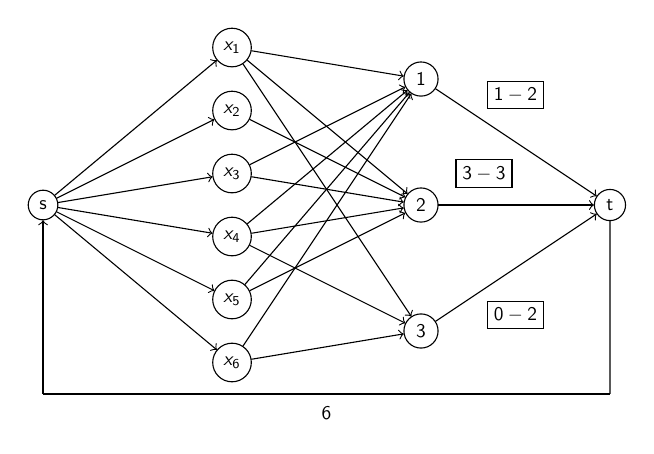
\begin{tikzpicture}[scale=0.8, every node/.style={scale=0.7}]
		\node[draw,circle] (s)at(0,0) {s};
		\node[draw,circle] (x1)at(3,2.5) {$x_1$};
		\node[draw,circle] (x2)at(3,1.5) {$x_2$};
		\node[draw,circle] (x3)at(3,0.5) {$x_3$};
		\node[draw,circle] (x4)at(3,-0.5) {$x_4$};
		\node[draw,circle] (x5)at(3,-1.5) {$x_5$};
		\node[draw,circle] (x6)at(3,-2.5) {$x_6$};
		\node[draw,circle] (y1)at(6,2) {1};
		\node[draw,circle] (y2)at(6,0) {2};
		\node[draw,circle] (y3)at(6,-2) {3};
		\node[draw,circle] (t)at(9,0) {t};
		\draw[->] (s) --(x1);
		\draw[->] (s) -- (x2);
		\draw[->] (s) -- (x3);
		\draw[->] (s) -- (x4);
		\draw[->](s) -- (x5);
		\draw[->] (s) -- (x6);
		\draw[->] (x1) -- (y1);
		\draw[->] (x1) -- (y2);
		\draw[->] (x1) -- (y3);
		\draw[->] (x2) -- (y2);
		\draw[->] (x3) -- (y1);
		\draw[->] (x3) -- (y2);
		\draw[->] (x4) -- (y1);
		\draw[->] (x4) -- (y2);
		\draw[->] (x4) -- (y3);
		\draw[->] (x5) -- (y1);
		\draw[->] (x5) -- (y2);
		\draw[->] (x6) -- (y1);
		\draw[->] (x6) -- (y3);
		\draw[->] (y1) -- (t);
		\draw[->] (y2) -- (t);
		\draw[->] (y3) -- (t);
		
		\draw (t)--(9,-3);
		\draw (9,-3)--(0,-3);
		\draw[->](0,-3)--(s);
		\node (loop) at (4.5,-3.3) {$6$};
		
		\node[draw] (bound1) at (7.5,1.75) {$1-2$};
		\node[draw] (bound2) at (7,0.5) {$3-3$};
		\node[draw] (bound3) at (7.5,-1.75) {$0-2$};
		
		\end{tikzpicture}
		
		\caption{Flow model of the instance of gcc presented in Example \ref{Examplegcc}}
		\label{flowproblemexample}
	\end{figure}
    
    The labels $l_j-u_j$ between each value node $y_j$ and the sink $t$ represent the lower bound and upper bound for the flow between $y_j$ and $t$. In order to make Figure \ref{flowproblemexample} easier to read, we did not represent the labels for edges between variables and values and between the source $s$ and the variables. The flow between a variable and a value must be $0$ or $1$ and the flow between the source $s$ and each variable is $1$.
	
	Then $(1,2,1,2,2,3)$ and $(3,2,1,2,2,3)$ are solutions but $(1,2,1,1,2,3)$ is not because the value $2$ is only taken twice and it must be taken at least three times.
	\label{Examplegcc}
\end{example}


\subsection{Matching Theory}
\label{matchingbackground}
We will see in subsection~\ref{stateoftheartPesant} that the global cardinality constraint can also be modeled as a maximum matching problem. The next definitions recall some graph and matching theory definitions that will be used afterwards. In the following, we will consider an undirected bipartite graph written $G=(V,E)$ for a graph, and $V = V_1 \cup V_2$ the two subsets of nodes corresponding to the \minor{partitions} of $G$. The graph $G$ is balanced iff $|V_1|=|V_2|$. Unless specified, we take the same framework and notations as \cite{MT09} and we refer the reader to this book for more details.

\begin{definition}[Biadjacency matrix of a bipartite graph %\cite{MT09} p.307
]
	Let $G(V_1 \cup V_2, E)$ be an undirected bipartite graph. We call the biadjacency matrix of $G$, the matrix $B_G=(b_{ij})$ such that
	\begin{equation}
		b_{ij} = \colon\begin{cases}
							1, \text{if } (v_i,v_j) \in E \text{ with } v_i \in V_1 \text{ and } v_j \in V_2 \\
							0, \text{otherwise}
						\end{cases}
\end{equation}
\end{definition}

\begin{definition}[Matching%\cite{MT09} xxxii
]
Let $G(V,E)$ and $M \subseteq E$. $M$ is a matching on $G$ iff no two edges of $M$ have a node in common.
\end{definition}

\begin{definition}[Maximum matching%, \cite{MT09} p.2
]
Let $G(V,E)$ and $M \subseteq E$. $M$ is a maximum matching on $G$  iff $M$ is a matching on $G$ and $|M|$ is maximum.%$M$ covers the greatest number of nodes.
\end{definition}

\begin{definition}[Perfect matching%, \cite{MT09} p.6
]
Let $G(V_1\cup V_2,E)$ and $M \subseteq E$. $M$ is a perfect matching on $G$ if and only iff $M$ is a matching on $G$ and $|M|=|V_1|=|V_2|$.%$M$ covers every node of $G$.
\end{definition}

\paragraph{}
Note that a perfect matching can only exist in a balanced graph. Also, a perfect matching is a maximum matching. We note $\#PM(G)$, the number of perfect matchings in $G$.

The next definition and proposition are the main results that \cite{PesantQZ12} have shown to be relevant to count solutions on a global cardinality constraint. \minor{In the following, we write $\mathbb{M}_{n,n}$ the set of square matrices of size $n$ and $S_n$, the symmetry group over $\lbrace 1, \ldots, n \rbrace$, that is the group of permutations over $\lbrace 1, \ldots, n \rbrace$}.

\begin{definition}[Permanent of a matrix%, \cite{MT09} p.309
]
	Let $A=(a_{ij}) \in \mathbb{M}_{n,n}$ \minor{be} a square matrix, \minor{we define the permanent of $A$ a follow:}
	\begin{equation}
		\perm{A} = \underset{\sigma \in S_n}{\sum}\prod_{i=1}^n a_{i,\sigma(i)}
	\end{equation}
	is the permanent of A.
\end{definition}

\paragraph{}
The permanent of a matrix looks similar to the determinant of a matrix. However, it is much harder to compute. It is actually a $\#P-$complete problem, as explained in \cite{Valiant79}.

\begin{proposition}%[\cite{MT09} p.309-310]
	Let $G(V_1 \cup V_2, E)$ be a balanced bipartite graph and $B_G$ \minor{be} its biadjacency matrix, then the number of perfect matchings in $G$ is equal to the permanent of $B_G$:
	\begin{equation}
		\perm{B_G}=\nbperfectmatching{G}
	\end{equation}
\end{proposition}
This result is given in \cite{MT09} and we will not detail its proof. Actually, a perfect matching in $G$ corresponds to a permutation $\sigma \in \mathcal{S}_n$ such that, $\forall i \in \lbrace 1, \ldots, n \rbrace$, $b_{i\sigma(i)} = 1$, where $B_G = (b_{ij})$ is the biadjacency matrix of $G$. This result is central in this study, as it gives a mathematical way to compute the number of perfect matchings in a balanced bipartite graph. Since the exact computation of $\perm{B_G}$ is $\#P$-complete, we will use two  upper bounds that can be computed in polynomial time.
	
	The first one is the Br\'egman-Minc upper bound conjectured in~\cite{Minc63} and proven in~\cite{Bregman73}.
\begin{proposition}[Br\'egman-Minc upper bound]
Let $A \in \mathbb{M}_{n,n}$ and $\forall \fromto{i}{1}{n}, r_i$ the sum of the $i^{th}$ row of $A$, then
\begin{equation}
	\perm{A} \leq \bregmanmincbound{A} = \prod_{i=1}^n (r_i!)^{\frac{1}{r_i}}
\end{equation}
\end{proposition}

The second one is the Liang-Bai upper bound established in~\cite{LiangB04}. An independent proof of this bound has been published in~\cite{Friedland08} .
\begin{proposition}[Liang-Bai upper bound]
Let $A \in \mathbb{M}_{n,n}$ and $\forall \fromto{i}{1}{n}, r_i$ the sum of the $i^{th}$ row of $A$ and $q_i=min(\lceil \frac{r_i+1}{2} \rceil, \lceil \frac{i}{2} \rceil )$, then
\begin{equation}
	\perm{A} \leq \liangbaibound{A} = \prod_{i=1}^n \sqrt {q_i(r_i-q_i+1)}
\end{equation}	
\end{proposition}
 
None of these bounds strictly dominates the other. In the following, $\bregmanmincbound{B_G}$ can also be noted as $\bregmanmincbound{G}$ (same for $\liangbaibound{B_G}$), where $B_G$ is biadjacency matrix of $G$.


\section{Counting the Solutions to a Global Cardinality Constraint}
\label{errorStateoftheart}

In this section, we present the method proposed in \cite{PesantQZ12} to compute an upper bound on the number of solutions of a $gcc$ instance. This method requires to compute the number of maximum matchings covering one \minor{partition} of an unbalanced bipartite graph. Subsection \ref{unbalancedbipartitegraph} presents how \cite{PesantQZ12} suggests to enumerate those maximum matchings. The method is then described in Subsection \ref{stateoftheartPesant} before we develop a counter-example to prove it wrong in Subsection \ref{counter-example}. Subsection \ref{RefiningProblem} introduces a new model that will help us \minor{in} fixing the error. 


\subsection{Number of maximum matchings of an unbalanced bipartite graph}
\label{unbalancedbipartitegraph}
We have seen how to count the number of perfect matchings on a balanced bipartite graph. For unbalanced bipartite graph, we are interested in counting the number of maximum matchings that cover every node of the smaller \minor{partition}. In the following, if $G$ is not balanced, then $\nbperfectmatching{G}$ refers to the number of maximum matchings that cover the smaller \minor{partition}.

We present here the way \cite{PesantQZ12} use to deal with unbalanced graphs.
Let us consider $G(V_1 \cup V_2, E)$, such that $|V_1| < |V_2|$. We are interested in computing the number of matching covering every node in $V_1$. In order to retrieve a balanced graph, first, $n_f$ fake nodes are added to \minor{partition} $V_1$.% in order to balance the bipartite graph. 

\begin{notation}
	If $G$ is an unbalanced bipartite graph, we note $G^{bal}$ the corresponding balanced bipartite graph, after adding the fake nodes.
\end{notation}


After balancing the graph, the number of perfect matchings on $G^{bal}$ can be computed, as seen in subsection \ref{matchingbackground}. Since there are fake nodes, the computed permanent (or upper bound) is an overestimation of the true number of matching covering $V_1$ on $G$. \cite{PesantQZ12} proposes to divide the permanent of the balanced graph by the number of permutations among the fake nodes. Indeed, for each matching covering $V_1$ on $G$, there are $n_f!$ corresponding perfect matchings on $G^{bal}$, each fake node being linked to every node in $V_2$. 
In the following, if $G$ is not balanced, $\#PM(G)$ refers to the number of maximum matchings covering the smaller \minor{partition} and we can write $\#PM(G) = \frac{\#PM(G^{bal})}{n_f!}$. Also, we will consider that $UB^{BM}(G)$ is an upper bound over the number of maximum matchings and $UB^{BM}(G) = \frac{UB^{BM}(G^{bal})}{n_f!}$ (same thing for $UB^{LB}(G)$).

A practical case of this method is developed in Example \ref{FirstExample}.


\subsection{ Upper bounding the number of solutions to a gcc}
\label{stateoftheartPesant}
We present here the method proposed in~\cite{PesantQZ12} to compute an upper bound of the number of solutions of a $gcc$ instance. The authors first count partial instantiations that satisfy the lower bound restriction. Then, for each of these partial instantiations, they count how many possibilities there are to complete it to a full instantiation satisfying the upper bound restriction.

\cite{PesantQZ12} only considers instances in which every fixed variable (that can be instantiated to only one value) has been removed and the lower and upper bound have been adjusted accordingly. Let $ \adjustedX = \lbrace \var{i} \in X | \; \var{} \; \text{is not fixed} \rbrace$ \minor{be} the set of unfixed variables and lower bounds are $\adjustedlow$ where $\adjustedlow_d = \low_d-|\lbrace \var{i} | \var{i} \text{ is fixed and } d \in D_i \rbrace|$ and upper bounds $\adjustedup$ are defined similarly. We assume that, $\forall d \in D_X$, $l'_d \geq 0$ and $u'_d \geq 0$.

The first stage of the method counts the partial instantiations satisfying the lower bound restriction. For this purpose, the notion of \emph{Lower Bound Graph} is introduced:
	
\begin{definition}[Lower Bound Graph, \cite{PesantQZ12}]
Let $\lowerboundgraph (\adjustedX \cup \Domain_l, E_l )$ be an undirected bipartite graph where $\adjustedX$ is the set of unfixed variables and $\Domain_l$, the extended value set, that is for each $d \in \DX$ the graph has $\adjustedlow_d$ vertices $d^1,d^2, \ldots$ representing $d$ ($\adjustedlow_d$ possibly equal to zero). There is an edge $(\var{i}, d^k) \in E_l$ if and only if $d \in \domainof{i}$.
\end{definition}

Figure~\ref{BoundGraph}a represents the Lower Bound Graph for the instance described in Example \ref{Examplegcc} and its computation is detailed in Example \ref{FirstExample}.

\begin{figure}
\centering
	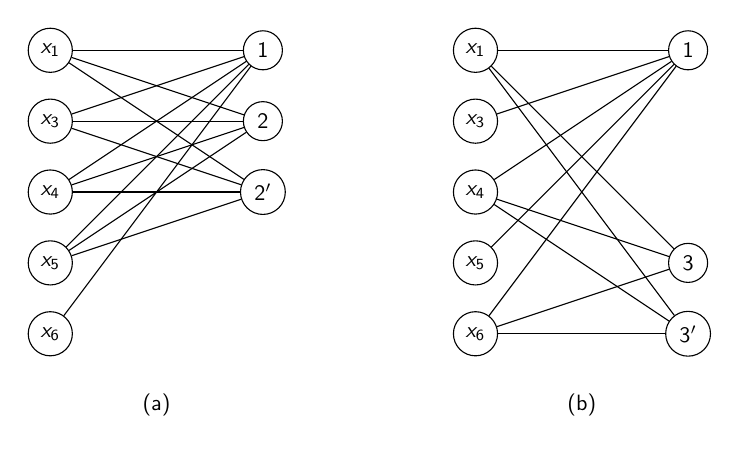
\begin{tikzpicture}[scale=0.9, every node/.style={scale=0.8}]
		\node[draw,circle] (x1a)at(0,0) {$x_1$};
		\node[draw,circle] (x3a)at(0,-1) {$x_3$};
		\node[draw,circle] (x4a)at(0,-2) {$x_4$};
		\node[draw,circle] (x5a)at(0,-3) {$x_5$};
		\node[draw,circle] (x6a)at(0,-4) {$x_6$};
		\node[draw,circle] (y1a)at(3,0) {$1$};
		\node[draw,circle] (y21a)at(3,-1) {$2$};
		\node[draw,circle] (y22a)at(3,-2) {$2'$};
		\node(figurea)at(1.5,-5){(a)};
		\draw (x1a) -- (y1a);
		\draw (x1a) -- (y21a);
		\draw (x1a) -- (y22a);
		\draw (x3a) -- (y1a);
		\draw (x3a) -- (y21a);
		\draw (x3a) -- (y22a);
		\draw (x4a) -- (y1a);
		\draw (x4a) -- (y21a);
		\draw (x4a)-- (y22a);
		\draw (x5a) -- (y1a);
		\draw (x5a) -- (y21a);
		\draw (x5a) -- (y22a);
		\draw (x6a) -- (y1a);
		
		\node[draw,circle] (x1b)at(6,0) {$x_1$};
		\node[draw,circle] (x3b)at(6,-1) {$x_3$};
		\node[draw,circle] (x4b)at(6,-2) {$x_4$};
		\node[draw,circle] (x5b)at(6,-3) {$x_5$};
		\node[draw,circle] (x6b)at(6,-4) {$x_6$};
		\node[draw,circle] (y1b)at(9,0) {$1$};
		\node[draw,circle] (y31b)at(9,-3) {$3$};
		\node[draw,circle] (y32b)at(9,-4) {$3'$};
		\node(figurea)at(7.5,-5){(b)};
		\draw (y1b) -- (x1b);
		\draw (y1b) -- (x3b);
		\draw (y1b) -- (x4b);
		\draw (y1b) -- (x5b);
		\draw (y1b) -- (x6b);
		\draw (y31b) -- (x1b);
		\draw (y31b) -- (x4b);
		\draw (y31b) -- (x6b);
		\draw (y32b) -- (x1b);
		\draw (y32b) -- (x4b);
		\draw (y32b) -- (x6b);
	\end{tikzpicture}
	\caption{Lower Bound Graph (a) and Upper Bound Residual Graph (b) of the $gcc$ instance described in Example \ref{Examplegcc}}
	\label{BoundGraph}
\end{figure}

By construction, a matching covering every vertex of $D_l$ corresponds to a partial instantiation of the variables satisfying the lower bound restriction. The matching $\lbrace (x_1,2),(x_4,2'), \\ (x_5,1)\rbrace$ corresponds to the partial assignment $(2,2,\_,2,1,\_)$ ($x_2$ is already instantiated) and this partial instantiation satisfies the lower bound restriction. Note that the matching $\lbrace (x_1,2'),(x_4,2),(x_5,1)\rbrace$ leads to the same partial instantiation. Switching two duplicated values does not change the resulting partial instantiation. Actually, every combination of permutations among duplicates of a same value must be considered. There are $\frac{\#PM(G_l)}{\prod_{d \in D_X} l'_d !}$ partial instantiations satisfying the lower bound restriction.

The authors are now interested in counting every possibility to complete a partial instantiation to a full instantiation. Similarly, the Upper Bound Residual Graph is introduced:

\begin{definition}[Upper Bound Residual Graph, \cite{PesantQZ12}]
Let $\upperboundresidualgraph(\adjustedX \cup \Domain_u, E_u)$ be an undirected bipartite graph where $\adjustedX$ is the set of unfixed variables and $\Domain_u$ the extended value set, that is for each $d \in \DX$, the graph has $\adjustedup_d-\adjustedlow_d$ vertices $d^1,d^2,...$ representing $d$ (if $\adjustedup_d-\adjustedlow_d$ is equal to zero then there is no  vertex representing $d$). There is an edge $(\var{i}, d^k) \in E_u$ if and only if $d \in \domainof{i}$ and $\adjustedup_d-\adjustedlow_d > 0$.
\end{definition}

Figure~\ref{BoundGraph}b represents the Upper Bound Residual Upper Graph for the instance described in Example \ref{Examplegcc}. 
At this point, $K=\underset{d \in \DX}{\sum} \adjustedlow_d$ variables are already instantiated (without counting fixed variables). They are removed from the Upper Bound Residual Graph and, by construction, a matching covering the remaining variables corresponds to a completion of the partial assignment. On the partial instantiation $(2,2,\_,2,1,\_)$,  $x_3$ and $x_6$ remain to instantiate. The matching $\lbrace (x_3,1),(x_6,3') \rbrace$ leads to the full instantiation $(2,2,1,2,1,3)$, which satisfies both the lower bound and upper bound restrictions.

However, in general, there is an exponential number of partial assignments satisfying the lower bound restriction. It is not reasonable to compute the number of maximum matchings on $G_u$ for each of them.
\cite{PesantQZ12} suggests an over-approximation of the number of possibilities to complete each partial assignment: the $K$ variables already instantiated are the variables that contribute the less to the combinatorial complexity of the problem.
They remove the $K$ variables such that the number of maximum matchings in $G_u$ covering the remaining variables is maximized. The resulting graph is noted $\overline{G_u}$ (see Figure \ref{BoundGraph2}). Like in the Lower Bound Graph, there are symmetries among duplicated values in $D_u$. There are at most $\frac{\#PM(\overline{G_u})}{\prod_{d \in D_X} (u'_d-l'_d)!}$ ways to complete a partial instantiation satisfying the lower bound restriction to a full instantiation also satisfying the upper bound restriction.

\cite{PesantQZ12} concludes on the following upper bound:

\begin{equation}
	\#gcc(X,l,u) \leq \frac{\#PM(G_l) \cdot \#PM(\overline{G_u})}{\prod_{d \in D_X} l'_d! \cdot (u'_d -l'_d)!}
	\label{WrongBound}
\end{equation}

\paragraph{}
In practice, we do not compute directly the number of perfect matchings, but we use the Bregman-Minc or Liang-Bai upper bound (Subsection \ref{matchingbackground}). Also we do not compute exactly $\overline{G_u}$, because it would require to consider $\binom{|X'|}{K}$ graphs and to compute the number of perfect matchings for each of them. Instead, we remove the $K$ variables that contribute the less to the computation of the Bregman-Minc or Liang-Bai upper bound (\textit{i.e.} the ones having the smaller factors in the product).
Example \ref{FirstExample} details this method:


\begin{figure}
	\centering
	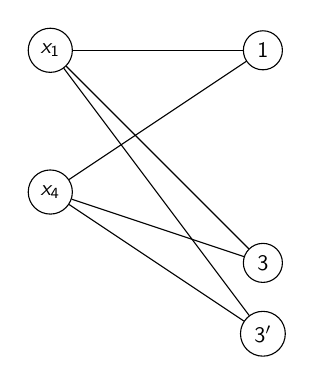
\begin{tikzpicture}[scale=0.9, every node/.style={scale=0.8}]
		\node[draw,circle] (x1)at(0,0) {$x_1$};
		\node[draw,circle] (x4)at(0,-2) {$x_4$};
		\node[draw,circle] (y1)at(3,0) {$1$};
		\node[draw,circle] (y31)at(3,-3) {$3$};
		\node[draw,circle] (y32)at(3,-4) {$3'$};
		\draw (x1) -- (y1);
		\draw (x1) -- (y31);
		\draw (x1) -- (y32);
		\draw (x4) -- (y1);
		\draw (x4) -- (y31);
		\draw (x4) -- (y32);
	\end{tikzpicture}
	\caption{Upper Bound Residual Graph after removing $x_3, x_5$ and $x6$ : $\overline{G_u}$}
	\label{BoundGraph2}
\end{figure}

\begin{example}
\label{FirstExample}
	We consider the same gcc as in Example \ref{Examplegcc}: $X = \setofVars{1}{6}$ with domains $\Domain_1=\Domain_4=\lbrace 1,2,3\rbrace, \Domain_2=\lbrace 2 \rbrace, \Domain_3=\Domain_5=\lbrace 1,2 \rbrace$ and $\Domain_6= \lbrace 1,3 \rbrace$; lower and upper bounds for the values are respectively $\low_1=1, \low_2=3, \low_3=0$ and $\up_1=2, \up_2=3 \up_3=2$. 
	
	Considering that $\var{2}=2$, the lower and upper bounds for the value 2 are respectively $\adjustedlow_2=2$ and $\adjustedup_2=2$. The Lower Bound Graph is shown in Figure 2a: variable $\var{2}$ is fixed and thus does not appear in the graph, value vertex 2 is represented by two vertices because $\adjustedlow_2=2$ ; finally value vertex 3 does not appear because $l'_3=0$. We construct similarly the Upper Bound Residual Graph (Figure \ref{BoundGraph}b).

We already have instantiated 3 variables at this stage (4, if we count $x_2$, which is fixed). To construct $\overline{G_u}$, we remove $x_3$, $x_5$ and $x_6$ from $G_u$, which contribute the less in the combinatorial complexity of the problem (we actually could have chosen $x_1$ or $x_4$ instead of $x_6$). $\overline{G_u}$ is such as in Figure \ref{BoundGraph2}.



First, we compute $\#PM(G_l)$. We add two fake vertices on the value \minor{partition}, $v$ and $v'$, in order to balance $G_l$ (Figure \ref{LBGbal}) and we compute the permanent of its biadjacency matrix (Figure \ref{BiadjacencymatrixOfLBG}). The permanent of $B_{G^{bal}_l}$ is 72. Then we divide by $2!$ to deal with the combinatorial complexity induced by the fake vertices, there are then $\#PM(G_l)=36$ matching covering the value \minor{partition} in $G_l$.

\begin{figure*}
\centering

\begin{subfigure}[normal]{0.4\textwidth}
\centering
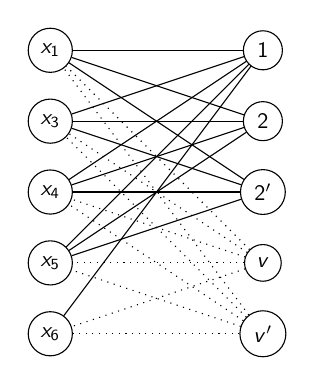
\begin{tikzpicture}[scale=0.9, every node/.style={scale=0.8}]
		\node[draw,circle] (x1a)at(0,0) {$x_1$};
		\node[draw,circle] (x3a)at(0,-1) {$x_3$};
		\node[draw,circle] (x4a)at(0,-2) {$x_4$};
		\node[draw,circle] (x5a)at(0,-3) {$x_5$};
		\node[draw,circle] (x6a)at(0,-4) {$x_6$};
		\node[draw,circle] (y1a)at(3,0) {$1$};
		\node[draw,circle] (y21a)at(3,-1) {$2$};
		\node[draw,circle] (y22a)at(3,-2) {$2'$};
		\node[draw,circle] (v)at(3,-3) {$v$};
		\node[draw,circle] (v2)at(3,-4) {$v'$};
		\draw (x1a) -- (y1a);
		\draw (x1a) -- (y21a);
		\draw (x1a) -- (y22a);
		\draw (x3a) -- (y1a);
		\draw (x3a) -- (y21a);
		\draw (x3a) -- (y22a);
		\draw (x4a) -- (y1a);
		\draw (x4a) -- (y21a);
		\draw (x4a) -- (y22a);
		\draw (x5a) -- (y1a);
		\draw (x5a) -- (y21a);
		\draw (x5a) -- (y22a);
		\draw (x6a) -- (y1a);
		\draw[dotted](v)--(x1a);
		\draw[dotted](v)--(x3a);
		\draw[dotted](v)--(x4a);
		\draw[dotted](v)--(x5a);
		\draw[dotted](v)--(x6a);
		
		\draw[dotted](v2)--(x1a);
		\draw[dotted](v2)--(x3a);
		\draw[dotted](v2)--(x4a);
		\draw[dotted](v2)--(x5a);
		\draw[dotted](v2)--(x6a);
		
		\end{tikzpicture}
        \caption{Lower Bound Graph after adding fake vertices, $G^{bal}_l$}
	\label{LBGbal}
\end{subfigure}
\hspace{2cm}
\begin{subfigure}[normal]{0.2\textwidth}
	\centering
     \vspace{1.8cm}
		$
	\begin{pmatrix}
		1 & 1 & 1 & 1 & 1 \\
		1 & 1 & 1 & 1 & 1 \\
		1 & 1 & 1 & 1 & 1 \\
		1 & 1 & 1 & 1 & 1 \\
		1 & 0 & 0 & 1 & 1 \\
	\end{pmatrix}
		$
       
    \caption{Biadjacency matrix of $G^{bal}_l$}
	\label{BiadjacencymatrixOfLBG}
\end{subfigure}
\caption{Lower Bound Graph after adding fake vertices and its biadjacency matrix}
\end{figure*}

Similarly, we can compute $\#PM(\overline{G_u})=6$. Then, we can conclude that:

\begin{equation*}
	\#gcc(X,l,u) \leq \frac{36 \cdot 6 }{2! \cdot 2!} = 54
\end{equation*}

The true number of solutions of this problem is 19. Scaling and also fake vertices used with the permanent bounds are factors that degrade the quality of the upper bound.
\end{example}	


%--------------------------------------------------------------------------------------
%--------------------------------------------------------------------------------------
%--------------------------------------------------------------------------------------
%--------------------------------------------------------------------------------------
%--------------------------------------------------------------------------------------
%--------------------------------------------------------------------------------------

%--------------------------------------------------------------------------------------
%--------------------------------------------------------------------------------------
%--------------------------------------------------------------------------------------
%--------------------------------------------------------------------------------------
%--------------------------------------------------------------------------------------
%--------------------------------------------------------------------------------------

%--------------------------------------------------------------------------------------
%--------------------------------------------------------------------------------------
%--------------------------------------------------------------------------------------
%--------------------------------------------------------------------------------------
%--------------------------------------------------------------------------------------
%--------------------------------------------------------------------------------------

%--------------------------------------------------------------------------------------
%--------------------------------------------------------------------------------------
%--------------------------------------------------------------------------------------
%--------------------------------------------------------------------------------------
%--------------------------------------------------------------------------------------
%--------------------------------------------------------------------------------------
\begin{figure}
	\centering
	\begin{tabular}{|c|ccc|}
			\hline
			Instantiation & $x_1$ & $x_2$ & $x_3$ \\
			\hline
			$\iota_1$ & 1 & 2 & 1 \\
			$\iota_2$ &1 & 2 & 2 \\
			$\iota_3$ &1 & 3 & 1 \\
			$\iota_4$ &1 & 3 & 2 \\
			$\iota_5$ &2 & 2 & 1 \\
			$\iota_6$ &2 & 3 & 1 \\
			$\iota_7$ &3 & 2 & 1 \\
			$\iota_8$ &3 & 3 & 1 \\
			\hline
		\end{tabular}
	\caption{Array of every instantiation}
	\label{ListOfInstantiations}
	\end{figure}
    
\subsection{Counter-example}
\label{counter-example}
The method described in the subsection \ref{stateoftheartPesant} does not work in general. We develop here a counter-example that proves it wrong and we analyze the error.

Let $X=\lbrace x_1, x_2, x_3 \rbrace$, $ D_1=\lbrace 1,2,3 \rbrace$ , $D_2= \lbrace 2,3\rbrace$, $D_3= \lbrace 1,2\rbrace$ and $l=\lbrace 1,0,0 \rbrace$ and $u=\lbrace 2,3,2 \rbrace$. A list of every instantiation is given by Figure~\ref{ListOfInstantiations}.
	
The Lower Bound Graph and Upper Bound Residual Graph are presented by Figure~\ref{BoundGraphCounterExample}. \minor{Only value node "1" is in the Lower Bound Graph because $l_1=1, \; l_2=0 \text{ and } l_3=0$. Also the variable $x_2$ cannot take the value 1, this is why it is not in the Lower Bound Graph.} \minor{There is only one value in the Lower Bound Graph, which means that only one variable is instantiated at this stage, then we need to delete one variable from $G_u$. We choose to delete $x_3$, as this is the variable which have less impact on the combinatorial complexity. It ensures that we are computing an upper bound.} After deleting one variable from $G_u$, we have $\overline{G_u}$ presented by Figure~\ref{BoundGraphCounterExampleAfterDeletingVariables}.

	\begin{figure}
		\centering
		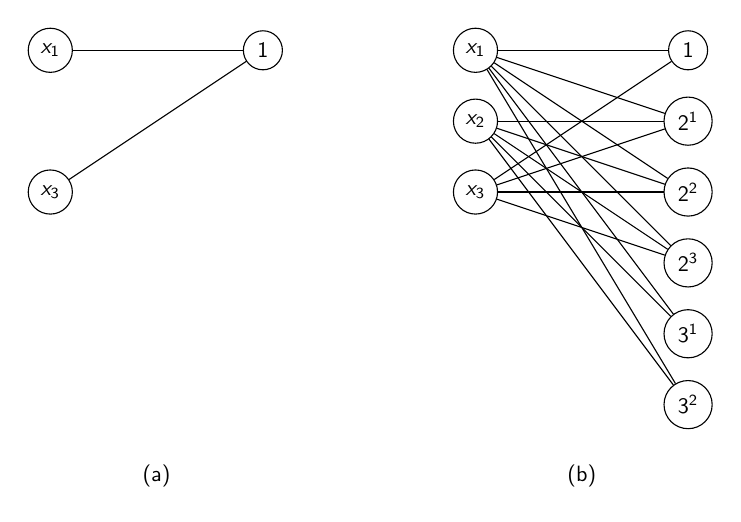
\begin{tikzpicture}[scale=0.9, every node/.style={scale=0.8}]
			\node[draw, circle] (x1a) at (0,0) {$x_1$};
			\node[draw, circle] (x3a) at (0,-2) {$x_3$};
			\node[draw, circle] (y1a) at (3,0) {$1$};
			\node (a)at(1.5,-6){(a)};
			\draw (x1a)--(y1a);
			\draw (x3a)--(y1a);
			

			\node[draw, circle] (x1) at (6,0) {$x_1$};
			\node[draw, circle] (x2) at (6,-1) {$x_2$};
			\node[draw, circle] (x3) at (6,-2) {$x_3$};
			\node[draw, circle] (y1) at (9,0) {$1$};
			\node[draw, circle] (y21) at (9,-1) {$2^1$};
			\node[draw, circle] (y22) at (9,-2) {$2^2$};
			\node[draw, circle] (y23) at (9,-3) {$2^3$};
			\node[draw, circle] (y31) at (9,-4) {$3^1$};
			\node[draw, circle] (y32) at (9,-5) {$3^2$};
			\node (b)at(7.5,-6){(b)};
			\draw (x1)--(y1);
			\draw (x1)--(y21);
			\draw (x1)--(y22);
			\draw (x1)--(y23);
			\draw (x1)--(y31);
			\draw (x1)--(y32);
			\draw (x2)--(y21);
			\draw (x2)--(y22);
			\draw (x2)--(y23);
			\draw (x2)--(y31);
			\draw (x2)--(y32);
			\draw (x3)--(y1);
			\draw (x3)--(y21);
			\draw (x3)--(y22);
			\draw (x3)--(y23);
					
			
		\end{tikzpicture}
		\caption{Lower Bound Graph $G_l$ (a) and Upper Bound Residual Graph $G_u$ (b)}
		\label{BoundGraphCounterExample}
	\end{figure}		
	
	\begin{figure}
		\centering
		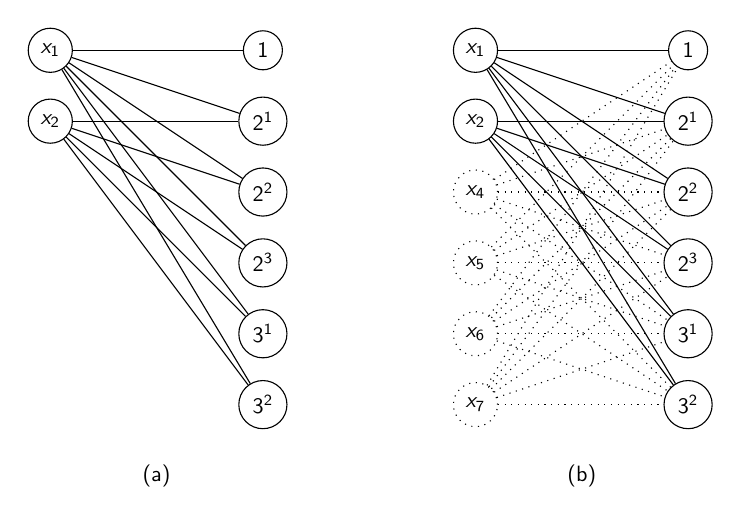
\begin{tikzpicture}[scale=0.9, every node/.style={scale=0.8}]
			\node[draw, circle] (x1) at (0,0) {$x_1$};
			\node[draw, circle] (x2) at (0,-1) {$x_2$};
			\node[draw, circle] (y1) at (3,0) {$1$};
			\node[draw, circle] (y21) at (3,-1) {$2^1$};
			\node[draw, circle] (y22) at (3,-2) {$2^2$};
			\node[draw, circle] (y23) at (3,-3) {$2^3$};
			\node[draw, circle] (y31) at (3,-4) {$3^1$};
			\node[draw, circle] (y32) at (3,-5) {$3^2$};
			\node (a)at(1.5,-6){(a)};
			\draw (x1)--(y1);
			\draw (x1)--(y21);
			\draw (x1)--(y22);
			\draw (x1)--(y23);
			\draw (x1)--(y31);
			\draw (x1)--(y32);
			\draw (x2)--(y21);
			\draw (x2)--(y22);
			\draw (x2)--(y23);
			\draw (x2)--(y31);
			\draw (x2)--(y32);					
			
			\node[draw, circle] (x1b) at (6,0) {$x_1$};
			\node[draw, circle] (x2b) at (6,-1) {$x_2$};
			\node[draw, circle,dotted] (x4b) at (6,-2) {$x_4$};
			\node[draw, circle,dotted] (x5b) at (6,-3) {$x_5$};
			\node[draw, circle, dotted] (x6b) at (6,-4) {$x_6$};
			\node[draw, circle, dotted] (x7b) at (6,-5) {$x_7$};
			\node[draw, circle] (y1b) at (9,0) {$1$};
			\node[draw, circle] (y21b) at (9,-1) {$2^1$};
			\node[draw, circle] (y22b) at (9,-2) {$2^2$};
			\node[draw, circle] (y23b) at (9,-3) {$2^3$};
			\node[draw, circle] (y31b) at (9,-4) {$3^1$};
			\node[draw, circle] (y32b) at (9,-5) {$3^2$};
			\node (b)at(7.5,-6){(b)};
			\draw (x1b)--(y1b);
			\draw (x1b)--(y21b);
			\draw (x1b)--(y22b);
			\draw (x1b)--(y23b);
			\draw (x1b)--(y31b);
			\draw (x1b)--(y32b);
			\draw (x2b)--(y21b);
			\draw (x2b)--(y22b);
			\draw (x2b)--(y23b);
			\draw (x2b)--(y31b);
			\draw (x2b)--(y32b);					
			
			\draw[dotted] (x4b)--(y1b);
			\draw[dotted] (x4b)--(y21b);
			\draw[dotted] (x4b)--(y22b);
			\draw[dotted] (x4b)--(y23b);
			\draw[dotted] (x4b)--(y31b);
			\draw[dotted] (x4b)--(y32b);
			
			\draw[dotted] (x5b)--(y1b);
			\draw[dotted] (x5b)--(y21b);
			\draw[dotted] (x5b)--(y22b);
			\draw[dotted] (x5b)--(y23b);
			\draw[dotted] (x5b)--(y31b);
			\draw[dotted] (x5b)--(y32b);
			
			\draw[dotted] (x6b)--(y1b);
			\draw[dotted] (x6b)--(y21b);
			\draw[dotted] (x6b)--(y22b);
			\draw[dotted] (x6b)--(y23b);
			\draw[dotted] (x6b)--(y31b);
			\draw[dotted] (x6b)--(y32b);
			
			\draw[dotted] (x7b)--(y1b);
			\draw[dotted] (x7b)--(y21b);
			\draw[dotted] (x7b)--(y22b);
			\draw[dotted] (x7b)--(y23b);
			\draw[dotted] (x7b)--(y31b);
			\draw[dotted] (x7b)--(y32b);
			
		\end{tikzpicture}
		\caption{$\overline{G_u}$ (a) and $\overline{G_u}^{bal}$ (b)}
		\label{BoundGraphCounterExampleAfterDeletingVariables}
	\end{figure}		
    
    \begin{figure}
    	\centering
     \vspace{1.8cm}
	\minor{	$
	\begin{pmatrix}
		1 & 1 & 1 & 1 & 1 \\
		0 & 1 & 1 & 1 & 1 \\
		1 & 1 & 1 & 1 & 1 \\
		1 & 1 & 1 & 1 & 1 \\
		1 & 1 & 1 & 1 & 1 \\
        1 & 1 & 1 & 1 & 1 \\
	\end{pmatrix}
		$ }
        \caption{\minor{Biadjacency matrix of $\overline{G_u}^{bal}$} (in counter-example)}
        \label{BiadjacencyCounterExample}
    \end{figure}
	
If we apply directly the upper bound of Equation (\ref{WrongBound}) (see subsection~\ref{stateoftheartPesant}), we have:
	
	\begin{equation*}
		\#gcc(X,l,u) \leq \frac{\#PM(G_l) \cdot \#PM(\overline{G_u})}{\prod_{d \in D_X} l'_d! \cdot (u'_d -l'_d)!} = \frac{2 \cdot 25}{2! \cdot 3!} = \frac{25}{6} = 4,1666
	\end{equation*}
    
\minor{It is obvious that $\#PM(G_l)=2$, as for $\#PM(G_u)$, we compute the permanent of the biadjacency matrix of $\overline{G_u}^{bal}$ (Figure \ref{BiadjacencyCounterExample}) , $Perm(\mathcal{B}(\overline{G_u}^{bal}))=600$, and, as we added 4 fake variables, we divide by $4!$. Thus, we get $\#PM(\overline{G_u})=\frac{600}{4!}=25$.}

But, we know that $\#gcc(X,l,u) = 8$, as we enumerated every instantiation in Figure \ref{ListOfInstantiations}. There is an error when computing the number of matchings covering $x_1$ and $x_2$ in $\overline{G_u}^{bal}$. Figure \ref{listPerfectMatching} lists every perfect matching of $\overline{G_u}$ corresponding to $\lbrace x_1 = 1, x_2=3 \rbrace$.

\begin{figure}
	\centering
	\begin{tabular}{|c|cccccc|}
 	 \hline
 		 Perfect Matching & $x_1$ & $x_2$ & $x_4$ & $x_5$ & $x_6$ & $x_7$ \\
 	 \hline
  		$\mu_1$ & $1$ & $3^1$ & $2^1$ & $2^2$ & $2^3$ & $3^2$ \\
  		$\mu_2$ & $1$& $3^1$ & $2^1$ & $2^3$ & $2^2$ & $3^2$ \\
  		$\mu_3$ & $1$& $3^1$ & $2^2$ & $2^1$ & $2^3$ & $3^2$ \\
  		$\vdots$ & $\vdots$  & $\vdots$  & $\vdots$  & $\vdots$  & $\vdots$ &  $\vdots$  \\
  		$\mu_{24}$ & $1$ & $3^1$ & $3^2$ & $2^3$ & $2^2$ & $2^1$ \\
  		$\mu_{25}$ & $1$ & $3^2$ & $2^1$ & $2^2$ & $2^3$ & $3^1$ \\
  		$\mu_{26}$ & $1$& $3^2$ & $2^1$ & $2^3$ & $2^2$ & $3^1$ \\
  		$\mu_{27}$ & $1$& $3^2$ & $2^2$ & $2^1$ & $2^3$ & $3^1$ \\
  		$\vdots$ & $\vdots$  & $\vdots$  & $\vdots$  & $\vdots$  & $\vdots$ &  $\vdots$  \\
  		$\mu_{48}$ & $1$ & $3^2$ & $3^1$ & $2^3$ & $2^2$ & $2^1$ \\
  	\hline
	\end{tabular}
	\caption{Array of every perfect matchings on $\overline{G_u}^{bal}$ }
	\label{listPerfectMatching}
\end{figure}
We can notice, for example, that $\mu_1$ and $\mu_2$ are symmetric by transposition of $x_5$ and $x_6$ and also by transposition of $2^2$ and $2^3$. In the method proposed, we first deal with the fake variables symmetry and then with the duplicated values symmetry. The symmetry between $\mu_1$ and $\mu_2$ is thus counted twice instead of once. Fake variables symmetry and duplicated values symmetry  may actually offset each other and should not be treated separately.
	
However, the problem does not appear for the Lower Bound Graph, as the number of variables is greater than or equal to the number of values (including the duplicates). In that case, the fake vertices symmetry comes from the same \minor{partition} than the duplicated values symmetry. It is then impossible to have two perfect matchings being symmetric in both ways. In section \ref{RefiningProblem}, we modify the model to fit the case where the duplicated values symmetry and fake variables symmetry are conflictual.

%---------------------------------------------------------------------------------------------------------------------
%---------------------------------------------------------------------------------------------------------------------
%---------------------------------------------------------------------------------------------------------------------
%---------------------------------------------------------------------------------------------------------------------
%---------------------------------------------------------------------------------------------------------------------
%---------------------------------------------------------------------------------------------------------------------
%---------------------------------------------------------------------------------------------------------------------
%---------------------------------------------------------------------------------------------------------------------
%---------------------------------------------------------------------------------------------------------------------
%---------------------------------------------------------------------------------------------------------------------
%---------------------------------------------------------------------------------------------------------------------
%---------------------------------------------------------------------------------------------------------------------
%---------------------------------------------------------------------------------------------------------------------
%---------------------------------------------------------------------------------------------------------------------
%---------------------------------------------------------------------------------------------------------------------
%---------------------------------------------------------------------------------------------------------------------
%---------------------------------------------------------------------------------------------------------------------
%---------------------------------------------------------------------------------------------------------------------
%---------------------------------------------------------------------------------------------------------------------
%---------------------------------------------------------------------------------------------------------------------
%---------------------------------------------------------------------------------------------------------------------
%---------------------------------------------------------------------------------------------------------------------
%---------------------------------------------------------------------------------------------------------------------
%---------------------------------------------------------------------------------------------------------------------
%---------------------------------------------------------------------------------------------------------------------
%---------------------------------------------------------------------------------------------------------------------
%---------------------------------------------------------------------------------------------------------------------
%---------------------------------------------------------------------------------------------------------------------
%---------------------------------------------------------------------------------------------------------------------
%---------------------------------------------------------------------------------------------------------------------
%---------------------------------------------------------------------------------------------------------------------
%---------------------------------------------------------------------------------------------------------------------
%---------------------------------------------------------------------------------------------------------------------

\subsection{A model that fits our specific problem }
\label{RefiningProblem}
In the previous subsection, we saw that the method does not work when there are fewer variables than duplicated values. In this subsection, we formally present and purify the problem to fit this case. This model and notations will be retained in the next sections.

As before, let $X=\lbrace \var{1}, \ldots, \var{n}\rbrace$ \minor{be} the set of variables. For $i \in \lbrace 1, \ldots, n \rbrace, D_i$ is the domain of $x_i$ and we note $D_X=\bigcup_{i=1}^n D_i = \lbrace y_1, \ldots, y_m \rbrace$. Let $\omega \in \N^m$ \minor{be} the  vector of occurrences, such that $\sum_{j=1}^m \omega_j \geq n$. In order to satisfy the global cardinality constraints, the variables of $X$ must be instantiated in such a way that each value $y_j \in D_X$ is taken at most $\omega_j$ times. As in previous works \cite{PesantQZ12} and in Section \ref{stateoftheartPesant}, in order to work with balanced bipartite graph,  we add fake variables that can take any value from $D_X$. Let $\overline{X} = \lbrace \var{n+1}, \ldots \var{n+n'} \rbrace$ \minor{be}  the set of fake variables, such that $n+n' = \sum_{j=1}^m \omega_j$ and $\forall \var{i} \in \overline{X}, \domainof{i}= D_X$. 
We introduce now the $\omega$-multiplied value graph, \minor{which is the value graph, in which each value node $y_j$ has been duplicated $\omega_j$ times}:

\begin{definition}[$\omega$-multiplied value graph]
	Let $G(X, \omega)=((X \cup \overline{X}) \cup \Domain_{\omega}, E_{\omega} )$ be the $\omega-$multiplied value graph with $E_{\omega} =\lbrace (\var{i},y_j^k) | y_j \in \domainof{i} \rbrace$ and $D_{\omega}=\lbrace y_1^1, \ldots y_1^{\omega_1}, \ldots , y_m^1, \ldots y_m^{\omega_m} \rbrace$.
\end{definition}

Figure \ref{omvaluegraph} represents the $\omega$-multiplied value graph for the instance described in Example \ref{exampleModelRefined}.
We will prove that, by construction, a perfect matching in the $\omega$-multiplied value graph, corresponds to an instantiation over $X$ satisfying the restriction on the occurrences. We first define formally the set of perfect matchings in $G(X, \omega)$ and the set of instantiations over $X$ satisfying the restriction on the occurrences:

\begin{definition}[Set of perfect matchings]
	We note $\mathcal{PM}(X, \omega)$, the set of perfect matchings in $G(X,\omega)$:
	\begin{align*}
		\mathcal{PM}(X, \omega) = \lbrace \lbrace e_1, \ldots,  e_{n+n'} \rbrace \subseteq E_{\omega} | \forall a,b &\text{ if } \minor{a \neq b,} \; e_a = (x_{i_a}, y_{j_a}^{k_a}) \text{ and } e_b = (x_{i_b}, y_{j_b}^{k_b}), \\
		&\text{ then } x_{i_a} \neq x_{i_b} \text{ and } y_{j_a}^{k_a} \neq y_{j_b}^{k_b} \rbrace
	\end{align*}
\end{definition}


\begin{definition}[Set of instantiations over $X$]
	We note $\mathcal{I}(X, \omega)$, the set of instantiations over $X$ that satisfy the restriction on the occurrences $\omega_j$:
	\begin{equation*}
		\mathcal{I}(X,\omega) = \lbrace (d_1, \ldots, d_n) | d_i \in D_i \text{ and } |\lbrace d_i | d_i=y_j \rbrace| \leq \omega_j \rbrace
	\end{equation*}
\end{definition}

 To simplify the notations, $\mathcal{PM}(X,\omega)$ and $\mathcal{I}(X,\omega)$ will be referred to as $\mathcal{PM}$ and $\mathcal{I}$, when there is no ambiguity on the considered instances. By construction of the $\omega$-multiplied value graph, a perfect matching of $\mathcal{PM}$ corresponds to an instantiation of $\mathcal{I}$:
 
 \begin{proposition}
 	Let $\mu = \lbrace (x_1, y_{j_1}^{k_1}), \ldots, (x_{n+n'}, y_{j_{n+n'}}^{k_{n+n'}}) \rbrace \in \mathcal{PM}$, then $\iota = (y_{j_1}^{k_1}, \ldots, y_{j_n}^{k_n})$ is an instantiation from $\mathcal{I}$.
 \end{proposition}
 
\begin{proof}
	Let $\mu = (e_1, \ldots, e_{n+n'}) \in \mathcal{PM}$. For a $i \in \lbrace 1,...,n+n' \rbrace$, we write the edge  $e_i$ as $e_i=(x_i, y_{j_i}^{k_i})$. Let $\iota = (d_1, \ldots, d_n)$, such that $\forall i \in \lbrace 1,...,n\rbrace, d_i = y_{j_i}^{k_i}$.
	
	We have $\forall i \in \lbrace 1, \ldots, n \rbrace,  e_i=(x_i, y_{j_i}^{k_i}) \in \mathcal{PM} \subseteq E_{\omega}$, thus $d_i = y_{j_i}^{k_i} \in D_i$.
	
	Also, for a $j \in \lbrace 1, \ldots, m \rbrace$, we have $| \lbrace e_i \in \mu | y_{j_i}^{k_i} = y_j \rbrace| = \omega_j$, since every value nodes is covered once in $\mu$ and there are $\omega_j$ duplicated nodes for each value. Then $\forall \mu' \subseteq \mu, |\lbrace e_i \in \mu' | y_{j_i}^{k_i} = y_j \rbrace| \leq \omega_j$ and, in particular, $|\lbrace e_i \in \lbrace e_1, \ldots e_n \rbrace | y_{j_i}^{k_i} = y_j \rbrace| \leq \omega_j$. As $\forall i \in \lbrace 1, \ldots, n\rbrace, d_i = y_{j_i}^{k_i}$, we can conclude $ \forall j \in \lbrace 1, \ldots, m \rbrace, |\lbrace d_i | d_i=y_j\rbrace| \leq \omega_j$. Then $\iota \in \mathcal{I}$
\end{proof} 

\begin{notation}
	Let $\mu \in \mathcal{PM}$, we note $\pi(\mu) = \iota$ the corresponding instantiation as introduced above. %the projection of $\mu$ on $\mathcal{I}$.
\end{notation}

Several perfect matchings can lead to a same instantiation. Yes, the size of $\mathcal{I}$ and the size of $\mathcal{PM}$ are correlated. \major{In next section, we present how to compute} an upper bound of $|\mathcal{I}|$.
%
Example \ref{exampleModelRefined} illustrates these new definitions and properties:

\begin{example}
Let $X=\lbrace x_1, x_2\rbrace, D_1= \lbrace 1,2 \rbrace, D_2=\lbrace 2,3\rbrace $, $\omega=\lbrace 2,1,2\rbrace$ and $\overline{X}=\lbrace x_3, x_4, x_5\rbrace$. Then we obtain the $\omega-$multiplied value graph in Figure \ref{omvaluegraph}. We also list every instantiation of $\mathcal{I}$ in Figure \ref{listInstantiations}.

$\lbrace (x_1, 1'), (x_2, 2), (x_3, 3'), (x_4,1), (x_5,3) \rbrace$ is a perfect matching that leads to the instantiation $\iota_1 = (1,2)$. $\iota_1$ is also reached by  $\lbrace (x_1, 1), (x_2, 2), (x_3, 3), (x_4,1'), (x_5,3') \rbrace$ and  \\ $\lbrace (x_1, 1'), (x_2, 2), (x_3, 3), (x_4,3'), (x_5,1) \rbrace$.
\begin{figure}
	\centering
    \begin{subfigure}{0.3\textwidth}
    	\centering
   			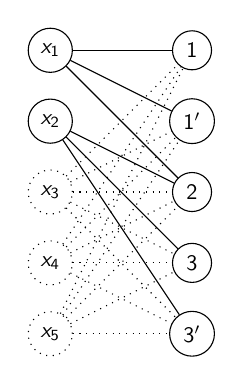
\begin{tikzpicture}[scale=0.9, every node/.style={scale=0.8}]
			 \node[draw,circle] (x1)at(0,0) {$x_1$};
			 \node[draw,circle] (x2)at(0,-1) {$x_2$};
			 \node[draw,circle,dotted] (x3)at(0,-2) {$x_3$};
			 \node[draw,circle,dotted] (x4)at(0,-3) {$x_4$};
			 \node[draw,circle,dotted] (x5)at(0,-4) {$x_5$};
			 \node[draw,circle] (y11)at(2,0) {$1$};
			 \node[draw,circle] (y12)at(2,-1) {$1'$};
			 \node[draw,circle] (y2)at(2,-2) {$2$};
			 \node[draw,circle] (y31)at(2,-3) {$3$};
			 \node[draw,circle] (y32)at(2,-4) {$3'$};
			 \draw (x1) -- (y11);
			 \draw (x1) -- (y12);
			 \draw (x1) -- (y2);
			 \draw (x2) -- (y31);
			 \draw (x2) -- (y32);
			 \draw (x2) -- (y2);
			 \draw (x3)[dotted]  -- (y11);
			 \draw (x3)[dotted] -- (y12);
			 \draw (x3)[dotted] -- (y2);
			 \draw (x3)[dotted] -- (y31);
			 \draw (x3)[dotted] -- (y32);
			 \draw (x4)[dotted] -- (y11);
			 \draw (x4)[dotted] -- (y12);
			 \draw (x4)[dotted] -- (y2);
			 \draw (x4)[dotted] -- (y31);
			 \draw (x4)[dotted] -- (y32);
			 \draw (x5)[dotted] -- (y11);
			 \draw (x5)[dotted] -- (y12);
			 \draw (x5)[dotted] -- (y2);
			 \draw (x5)[dotted] -- (y31);
			 \draw (x5)[dotted] -- (y32);
		\end{tikzpicture}
		\caption{$\omega-$multiplied Value Graph of the instance described in Example \ref{exampleModelRefined}}
		\label{omvaluegraph}
    \end{subfigure}
	\hspace{2cm}
    \begin{subfigure}{0.3\textwidth}
    \centering
    	\vspace{1.35cm}
		\begin{tabular}{ccc}
		instantiations & $x_1$ & $x_2$ \\
		\hline
		$\iota_1$ & 1 & 2 \\
		$\iota_2$ & 1 & 3 \\
		$\iota_3$ & 2 & 3 \\
		\end{tabular}
        \vspace{0.6cm}
		\caption{List of every elements of $\mathcal{I}$ for the Example \ref{exampleModelRefined}}
		\label{listInstantiations}
    \end{subfigure}
    \caption{$\omega$-multiplied value graph and list of every instantiation for Example \ref{exampleModelRefined}}
\end{figure}
\label{exampleModelRefined}
\end{example}

%---------------------------------------------------------------------------------------------------------------------
%---------------------------------------------------------------------------------------------------------------------
%---------------------------------------------------------------------------------------------------------------------
%---------------------------------------------------------------------------------------------------------------------
%---------------------------------------------------------------------------------------------------------------------
%---------------------------------------------------------------------------------------------------------------------
%---------------------------------------------------------------------------------------------------------------------
%---------------------------------------------------------------------------------------------------------------------
%---------------------------------------------------------------------------------------------------------------------
%---------------------------------------------------------------------------------------------------------------------
%---------------------------------------------------------------------------------------------------------------------
%---------------------------------------------------------------------------------------------------------------------
%---------------------------------------------------------------------------------------------------------------------
%---------------------------------------------------------------------------------------------------------------------
%---------------------------------------------------------------------------------------------------------------------
%---------------------------------------------------------------------------------------------------------------------
%---------------------------------------------------------------------------------------------------------------------
%---------------------------------------------------------------------------------------------------------------------
%---------------------------------------------------------------------------------------------------------------------
%---------------------------------------------------------------------------------------------------------------------
%---------------------------------------------------------------------------------------------------------------------
%---------------------------------------------------------------------------------------------------------------------
%---------------------------------------------------------------------------------------------------------------------
%---------------------------------------------------------------------------------------------------------------------
%---------------------------------------------------------------------------------------------------------------------
%----------------------------------------------------------------------------

\section{Upper-bound evaluation as a non\--linear minimization problem}

\major{This section introduces a correction for the bound proposed in \cite{PesantQZ12} and recalled in Section \ref{stateoftheartPesant}. Then we propose an algorithmic analysis of this correction}

\subsection{\major{A New Upper Bound}}
\label{calculatoryApproach}
Basically, the approach is to count how many perfect matchings in $G(X, \omega)$ lead to a specific instantiation, over the true variables, $\iota \in \mathcal{I}$. However, there are an exponential number of such instantiations, so we will find a lower bound of the number of such perfect matchings, by solving a non\--linear minimization problem, in order to upper bound the number of instantiations in $\mathcal{I}$.

\begin{proposition}
Let $\iota=(y_{j_1}, \ldots, y_{j_n})$ be an instantiation of $(\var{1}, ..., \var{n})$ and $\forall \fromto{j}{1}{m}$, $c_j(\iota)= |\lbrace i | y_{j_i}=y_j\rbrace|$, which are the number of occurrences of each value in $\iota$.
There are $n'! \cdot \prod_{j=1}^m A^{\omega_j}_{c_j(\iota)} $ perfect matchings on $G(X, \omega)$ that lead to the instantiation $\iota$, where $A^{\omega_j}_{c_j(\iota)}$ is the number of possible arrangements of $c_j(\iota)$ objects among $\omega_j$.
\label{nbPerfectMatchingleadingtoaninstantiation}
\end{proposition}

\begin{proof}
For each value $y_j \in \bigcup_{i=1}^n \Domain_i$, there are $\omega_j \choose c_j(\iota)$ ways to pick up nodes in $G$ to have as many occurrences of $y_j$ as in $\iota$ and there are $c_j(\iota)!$ ways to order these nodes, then there are $\binom{\omega_j}{c_j(\iota)} \cdot c_j(\iota)! = A^{\omega_j}_{c_j(\iota)}$  ways to assign variables of $X$ that are equal to $y_j$ in the instantiation $\iota$.

Each of these choices are independent, thus this result can be extended to every value $y_j$: there are $\underset{j\in \lbrace 1,...,m\rbrace}{\prod} A^{\omega_j}_{c_j(\iota)}$ ways to assign the variables in $X$ to get the instantiation $\iota$.

We need now to consider fake variables assignment. For each assignment of $X$ leading to the instantiation $\iota$, there are $n'!$ ways to assign every variable of $\overline{X}$, then, there are $n'! \cdot$ $\underset{j\in \lbrace 1,...,m\rbrace}{\prod} A^{\omega_j}_{c_j(\iota)}$ perfect matchings in $G(X, \omega)$, that lead to the instantiation $\iota$.
\end{proof}

The following example illustrates Proposition~\ref{nbPerfectMatchingleadingtoaninstantiation}.
\begin{example}
\label{examplenbinstantiations}
Let $X=\lbrace x_1, x_2\rbrace, D_1= \lbrace 1,2 \rbrace, D_2=\lbrace 2,3\rbrace $, and $\omega=\lbrace 2,1,2\rbrace$, then we must add 3 fake variables, $\overline{X}=\lbrace x_3, x_4, x_5\rbrace$. We obtain the $\omega-$multiplied value graph in Figure~\ref{omvaluegraph}.
\begin{figure}
	\centering
    \begin{subfigure}{0.2\textwidth}
     \vspace{1.6cm}
     \centering
    	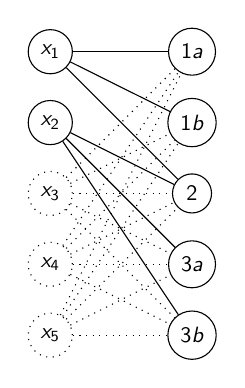
\begin{tikzpicture}[scale=0.9, every node/.style={scale=0.8}]
			 \node[draw,circle] (x1)at(0,0) {$x_1$};
			 \node[draw,circle] (x2)at(0,-1) {$x_2$};
			 \node[draw,circle,dotted] (x3)at(0,-2) {$x_3$};
			 \node[draw,circle,dotted] (x4)at(0,-3) {$x_4$};
			 \node[draw,circle,dotted] (x5)at(0,-4) {$x_5$};
			 \node[draw,circle] (y11)at(2,0) {$1a$};
			 \node[draw,circle] (y12)at(2,-1) {$1b$};
			 \node[draw,circle] (y2)at(2,-2) {$2$};
			 \node[draw,circle] (y31)at(2,-3) {$3a$};
			 \node[draw,circle] (y32)at(2,-4) {$3b$};
			 \draw (x1) -- (y11);
			 \draw (x1) -- (y12);
			 \draw (x1) -- (y2);
			 \draw (x2) -- (y31);
			 \draw (x2) -- (y32);
			 \draw (x2) -- (y2);
			 \draw (x3)[dotted]  -- (y11);
			 \draw (x3)[dotted] -- (y12);
			 \draw (x3)[dotted] -- (y2);
			 \draw (x3)[dotted] -- (y31);
			 \draw (x3)[dotted] -- (y32);
			 \draw (x4)[dotted] -- (y11);
			 \draw (x4)[dotted] -- (y12);
			 \draw (x4)[dotted] -- (y2);
			 \draw (x4)[dotted] -- (y31);
			 \draw (x4)[dotted] -- (y32);
			 \draw (x5)[dotted] -- (y11);
			 \draw (x5)[dotted] -- (y12);
			 \draw (x5)[dotted] -- (y2);
			 \draw (x5)[dotted] -- (y31);
			 \draw (x5)[dotted] -- (y32);
		\end{tikzpicture}
       
		\caption{$\omega-$multiplied Value Graph}
		\label{omvaluegraph2}
    \end{subfigure}
    \hspace{2cm}
    \begin{subfigure}{0.3\textwidth}
    \centering
		\begin{tabular}{ccccc}
		\hline
			$x_1$ & $x_2$ & $x_3$ & $x_4$ & $x_5$ \\
		\hline
			$1a$ & $2$ & $1b$ & $3a$ & $3b$ \\
			$1a$ & $2$ & $1b$ & $3b$ & $3a$ \\
			$1a$ & $2$ & $3a$ & $1b$ & $3b$ \\
			$1a$ & $2$ & $3a$ & $3b$ & $1b$ \\
			$1a$ & $2$ & $3b$ & $1b$ & $3a$ \\
			$1a$ & $2$ & $3b$ & $3a$ & $1b$ \\
			$1b$ & $2$ & $1a$ & $3a$ & $3b$ \\
			$1b$ & $2$ & $1a$ & $3b$ & $3a$ \\
			$1b$ & $2$ & $3a$ & $1a$ & $3b$ \\
			$1b$ & $2$ & $3a$ & $3b$ & $1a$ \\
			$1b$ & $2$ & $3b$ & $1a$ & $3a$ \\
			$1b$ & $2$ & $3b$ & $3a$ & $1a$ \\
		\hline
		\end{tabular}
		\caption{List of perfect matchings corresponding to the solution $\lbrace x_1=1, x_2=2 \rbrace$}
		\label{listperfectmatchingexample}
    \end{subfigure}
		\caption{$\omega$-multiplied graph and list of perfect matchings for Example \ref{examplenbinstantiations}}
\end{figure}
Let us now consider this instantiation of the variables $\var{1}$ and $\var{2}$ of this problem: $\lbrace x_1=1, x_2=2 \rbrace$, and let us call it $\iota$, we want to count how many perfect matching there are in $G(X, \omega)$ that lead to this instantiation. The array in Figure \ref{listperfectmatchingexample} lists those perfect matchings.
	 
Note that we can remove every symmetric perfect matching by permutation of the variables of $\overline{X}$. There are $3!=6$ such permutations. After deleting these perfect matchings, there remain 2 possibilities: either $\lbrace x_1=1a, x_2=2 \rbrace$ or $\lbrace x_1=1b, x_2=2 \rbrace$. In general, we need to count every possibility there is to instantiate variables in $X$. In $\iota$, we chose one value "1" among two, one value "2" among one and zero value "3" among two. Also the order in which we pick these values is important, then there are $3! \cdot A^2_1 \cdot A^1_1 \cdot A^2_0 = 12$  perfect matchings leading to the instantiation $\iota$.
\end{example}

We can directly deduce the following corollary, when extending Proposition~\ref{nbPerfectMatchingleadingtoaninstantiation} to every instantiation of $\mathcal{I}$:
\begin{corollary}
	\begin{equation}
	\nbperfectmatching{G(X, \omega)} = n'! \cdot \underset{\iota \in \mathcal{I}}{\sum} \prod_{j=1}^m A^{\omega_j}_{c_j(\iota)} 
	\end{equation}
	\label{corollary1}
\end{corollary}

The following proposition gives an upper bound for $|\mathcal{I}|$:
\begin{proposition}
	\begin{equation}
		|\mathcal{I}| \leq \frac{\nbperfectmatching{G(X,\omega)}}{n'! \cdot \underset{\iota \in \mathcal{I}}{min}(\prod_{j=1}^m A_{c_j(\iota)}^{\omega_j})}
	\end{equation}
\end{proposition}

\begin{proof}
The proof follows directly from Corollary \ref{corollary1}.
\end{proof}

\begin{remark}
What suggested the bound used in \cite{PesantQZ12} is that 
\begin{equation*}
		|\mathcal{I}| \leq \frac{\nbperfectmatching{G(X,\omega)}}{n'! \cdot \prod_{j=1}^m \omega_j!}
\end{equation*}
We can check that we have, $\forall \iota \in \mathcal{I}$,
\begin{equation*}
	\prod_{j=1}^m A_{c_j(\iota)}^{\omega_j} \leq \prod_{j=1}^m \omega_j!
\end{equation*}
and then,
\begin{equation*}
	\frac{\nbperfectmatching{G(X,\omega)}}{n'! \cdot \underset{\iota \in \mathcal{I}}{min}(\prod_{j=1}^m A_{c_j(\iota)}^{\omega_j})} \geq \frac{\nbperfectmatching{G(X,\omega)}}{n'! \cdot \prod_{j=1}^m \omega_j!}
\end{equation*}		
\end{remark}

Our new objective is to compute $\underset{\iota \in \mathcal{I}}{min}(\prod_{j=1}^m A_{c_j(\iota)}^{\omega_j})$. In the following, $c_j(\iota)$ will be just noted as $c_j$. This problem can be modeled as this minimization problem:
\begin{equation}
IP = \colon\begin{cases}
min \; \prod_{j=1}^m \frac{\omega_j !}{(\omega_j - c_j) !}\\
s.t. \sum_{j=1}^m c_j = n \\
\forall j \in \lbrace 1,...,m\rbrace, c_j \in \lbrace 0,..., \omega_j \rbrace
\end{cases}
\end{equation}

We can notice that for a high $\omega_j$, choosing a high $c_j$, makes the objective function rise much more than choosing a high $c_j$, for a small $\omega_j$. Also choosing a small $c_j$ for a high $\omega_j$ makes the objective function rise much more than choosing the same $c_j$ for a smaller $\omega_j$.

\begin{example}
Let $\omega_1=5$ and $\omega_2=2$ and $n=4$, then $c_1 \in [0,5]$ and $c_2 \in [0,2]$, then taking $c_1=4$ and $c_2=1$, for example, $\frac{5!}{(5-4)!}=120 > 2 = \frac{2!}{(2-2)!}$. \\	
And taking $c_1=1$ and $c_2=1$, we have $\frac{5!}{(5-1)!}=5 > 2= \frac{2!}{(2-1)!}$ \\
As we must satisfy $c_1+ c_2= n = 4$, it seems better to, first, assign the biggest value possible for $c_2$ and then assign the rest to $c_1$. We would have $c_1=2$ and $c_2=2$ and $A^2_2 * A^5_2 = 40$, which is the minimum.
\end{example}

This reasoning is generalized in the next proposition.
\begin{proposition}
If $\omega_1 \leq \ldots \leq \omega_m$, then $c^*=(\omega_1, \ldots, \omega_{k-1}, c^*_k, 0, \ldots, 0)$ is a minimum of $IP$, with $c^*_k = n-\sum_{j=1}^{k-1} \omega_j$.
\end{proposition}
\begin{proof}
Let $\omega = (\omega_1,...,\omega_m)$ and let consider that $\omega_1 \leq \cdots \leq \omega_m$ and 
\begin{equation}
f = \colon\begin{cases}
\N^m \rightarrow \N \\
c \mapsto \prod_{j=1}^m \frac{\omega_j !}{(\omega_j - c_j) !}\\
\end{cases}
\end{equation}
We want to minimize $f(c)$ such that $\sum_{j=1}^m c_j = n$. Then, $\omega$ being in ascending order, we want to prove that $f$ reaches a global minimum for:
\begin{equation}
 c^*=(\omega_1,...,\omega_{k-1}, c^*_k, 0,...,0) 
\end{equation}
with $c^*_k \in \lbrace 0,...,\omega_k \rbrace$.

Let $c=(c_1,...,c_m)$ be a vector such that $\sum_{j=1}^m c_j = n$. We want to prove that $f(c^*) \leq f(c)$. Let us rewrite $c$ as a modification of $c^*$. We can only decrease (not strictly) $c^*_j$ for $j \in \lbrace 1,..., k-1\rbrace$ and increase (not strictly) $c^*_j$ for $j \in \lbrace k+1,..., m\rbrace$. As for $c^*_k$, there are two possibilities. We first deal with the case where $c^*_k$ is increased. We rewrite $c$:
\begin{equation}
	c=(\omega_1-d_1, ..., \omega_{k-1}-d_{k-1}, \minor{c^*_k} +u_k, u_{k+1},...,u_m)
\end{equation}
with $\forall j \in \lbrace 1,...,m \rbrace, d_j \geq 0$ and $u_j \geq 0$ and $\sum_{j=1}^m u_j = \sum_{j=1}^m d_j$. We consider that $\forall j \in \lbrace k,...,m\rbrace , d_j=0$ and $\forall j \in \lbrace1,...,k-1 \rbrace, u_j=0$. The last condition states that everything that has been removed, has also been added. Thus, we still have $\sum_{j=1}^m c_j = n$.

Now, we will see a method to transform vector $c^*$ to $c$ in several steps such that, at every step, the function $f$ increases. Let $c^j$ be the vector at step $j$.

For each $j \in \lbrace 1, k-1\rbrace$, we remove $d_j$ from $c^j_j$, and we redistribute on the variables of the end, that need to be increased, starting redistributing from index $k$ to $m$. Let us take an example:

Let us consider a vector $\omega=(2,3,4,4,7)$ and $n=7$. Then, let $c^* = (2,3,2,0,0)$ and $c=(0,1,3,1,2)$. Here are the steps following the method to get $c$ from $c^*$:
	\begin{itemize}
		\item[-] Step 0: $c^0=c^*=(2,3,2,0,0)$
		\item[-] Step 1: $c^1=(0,3,3,1,0)$, we remove $2$ from $c^0_1$ and we add $1$ to $c^0_3$ and $1$ to $c^0_4$.
		\item[-] Step 2: $c^2=c=(0,1,3,1,2)$, we remove $2$ from $c^1_2$ and we add $2$ to $c^1_5$.
	\end{itemize}

In a general way, we have:
\begin{itemize}
	\item[-] Step 0: $c^0=c^*=(\omega_1, ..., \omega_{k-1}, c^*_k,0,...,0)$.
	\item[-] ...
	\item[-] Step j: $c^j=(\omega_1-d_1,..., \omega_j -d_j, \omega_{j+1},..., \omega_{k-1}, c^*_k + u_k, u_{k+1}, ..., u_{q-1}, r_q, 0, ...,0)$.
	\item[-] ...
	\item[-] Step k-1 : $c^{k-1}=c=(\omega_1-d_1,..., \omega_{k-1}-d_{k-1}, c^*_k +u_k, u_{k+1},..., u_m)$.
\end{itemize}
with $r_q \in \lbrace 1,...,u_q \rbrace$ (or $\lbrace x^*_k,..., x^*_k + u_k\rbrace$, if $q=k$), which is the residue for a particular index $q$. This index does not necessarily increase from one step $j$ to the following one, as $d_j$ may be smaller than $u_q-r_q$.

The objective, now, is to prove that $f(c^j) \leq f(c^{j+1}), \forall j \in \lbrace 1,...,k-2\rbrace$. We have:
\begin{equation*}
	c^j=(\omega_1-d_1,..., \omega_j -d_j, \omega_{j+1},..., \omega_{k-1}, c^*_k + u_k, u_{k+1}, ..., u_{q_a-1}, r_{q_a}, 0, ...,0)
\end{equation*}
and
\begin{equation*}
	c^{j+1}=(\omega_1-d_1,..., \omega_{j+1}-d_{j+1}, \omega_{j+2}..., \omega_{k-1}, c^*_k + u_k, u_{k+1}, ..., u_{q_b-1}, r_{q_b}, 0, ...,0)
\end{equation*}
with $q_b \geq q_a$.

Now, we study $\frac{f(c^j)}{f(c^{j+1})}$.

\paragraph{First case: $q_a < q_b$}
\begin{align*}
	\frac{f(c^j)}{f(c^{j+1})} &= \frac{\omega_{j+1}!}{\frac{\omega_{j+1}!}{d_{j+1}!}} \cdot \frac{\frac{\omega_{q_a}!}{(\omega_{q_a}-r_{q_a})!}}{\frac{\omega_{q_a}!}{(\omega_{q_a}-u_{q_a})!}} \cdot \frac{1}{\frac{\omega_{q_b}!}{(\omega_{q_b}-r_{q_b})!}} \\
	&= d_{j+1}! \cdot \frac{(\omega_{q_a}-u_{q_a})!}{(\omega_{q_a}-r_{q_a})!} \cdot \frac{(\omega_{q_b}-r_{q_b})!}{\omega_{q_b}!} \\
	&= \frac{ (d_{j+1}-r_{q_b})! \cdot (d_{j+1} - r_{q_b} +1) \cdot ... \cdot d_{j+1}}      {(\omega_{q_a}-r_{q_a}) \cdot ... \cdot (\omega_{q_a} - u_{q_a}+1) \cdot \omega_{q_b} \cdot ... \cdot (\omega_{q_b}-r_{q_b}+1)}
\end{align*}
And, $(d_{j+1} - r_{q_b} +1) \cdot ... \cdot d_{j+1}$ and $\omega_{q_b} \cdot ... \cdot (\omega_{q_b}-r_{q_b}+1)$ are products of $r_{q_b}$ consecutive terms. Moreover, $\omega_{q_b} \geq \omega_{j+1} \geq d_{j+1}$, then:
\begin{equation*}
	\frac{(d_{j+1} - r_{q_b} +1) \cdot ... \cdot d_{j+1}}{\omega_{q_b} \cdot ... \cdot (\omega_{q_b}-r_{q_b}+1)} \leq 1
\end{equation*}
We can notice that, in the case where redistributing $d_{j+1}$ makes the index of the residue grow, $d_{j+1} = (u_{q_a}-r_{q_a}) + r_{q_b}$. In other words, what has been removed has been re-added. Then $(d_{j+1}-r_{q_b})!$ is the product of $u_{q_a}-r_{q_b}$ consecutive terms, the same as $(\omega_{q_a}-r_{q_a}) \cdot ... \cdot (\omega_{q_a} - u_{q_a}+1)$. We also know that $\omega_{q_a} \geq u_{q_a}$, then $d_{j+1} - r_{q_b} = u_{q_a}-r_{q_a} \leq \omega_{q_a} - r_{q_a}$, then:
\begin{equation*}
	\frac{(d_{j+1}-r_{q_b})!}{(\omega_{q_a}-r_{q_a}) \cdot ... \cdot (\omega_{q_a} - u_{q_a}+1)} \leq 1
\end{equation*}
Then, 
\begin{equation*}
	\frac{f(c^j)}{f(c^{j+1})} \leq 1
\end{equation*}

\paragraph{Second case: $q_a=q_b$}
We consider here the case where the index of the residue remains unchanged, but this does not mean that the residue is the same for $c^j$ and $c^{j+1}$. Then we have $q_b = q_a$ and $r_{q_b} \geq r_{q_a}$. But we have $\omega_{q_a} = \omega_{q_b}$.
\begin{align*}
	\frac{f(c^j)}{f(c^{j+1})} &= d_{j+1}! \cdot \frac{\frac{\omega_{q_a}!}{(\omega_{q_a}-r_{q_a})!}}  {\frac{\omega_{q_b}!}{(\omega_{q_b}-r_{q_b})!}} \\
											&= d_{j+1}! \cdot \frac{(\omega_{q_b} - r_{q_b})!}{(\omega_{q_a} - r_{q_a})!} \\
											&= \frac{d_{j+1}!}{(\omega_{q_a}-r_{q_a}) \cdot... \cdot (\omega_{q_a} - r_{q_b} +1)}
\end{align*}
What has been removed, has also been re-added: $d_{j+1}=r_{q_b}-r_{q_a}$ then $d_{j+1}!$ is a product of $r_{q_b}-r_{q_a}$ consecutive terms, like the product $(\omega_{q_a}-r_{q_a}) \cdot... \cdot (\omega_{q_a} - r_{q_b} +1)$. Moreover, $d_{j+1}=r_{q_b}-r_{q_a} \leq \omega_{q_a} - r_{q_a}$. Thus we have,
\begin{equation*}
	\frac{f(c^j)}{f(c^{j+1})} \leq 1
\end{equation*}

We have proved that, $\forall j \in \lbrace 1,..., k-2 \rbrace$, $f(c^j) \leq f(c^{j+1})$. Then,
\begin{equation*}
	f(c^*)=f(c^0) \leq f(c^1) \leq ... \leq f(c^{k-1}) = f(c)
\end{equation*}

There remains one case to deal with. We have proved that $f(c^*) \leq f(c)$, for every $c$ such that $c_k \geq c^*_k $. In the case where $c_k \leq c^*_k$, we need to adapt the method described above. In the previous case, we started removing $d_j$ for $j$ going from $1$ to $k-1$ in that order. In this case, we first remove $d_k$ and only, then we remove $d_j$ for $j$ going from $1$ to $k-1$, as before.
We will not detail the calculations for this case as they are very similar. 

It follows that $f(c^*) \leq f(c)$ for every $c$ such that $\sum_{j=1}^m c_j=n$ and $\forall j \in \lbrace 1,...,m \rbrace, 0 \leq c_j \leq \omega_j$. Then $c^*$ is a minimum of our problem.
\end{proof}

From this proposition, we can deduce a method to get an upper bound of $\mathcal{I}$. We first sort the occurrences vector $\omega$, then we can compute the vector $c^*$ and compute $\underset{\iota \in \mathcal{I}}{min}(\prod_{j=1}^m A_{c_j(\iota)}^{\omega_j})=\prod_{j=1}^m A_{c^*_j}^{\omega_j}$. Then we get an upper bound of $|\mathcal{I}|$.
\begin{proposition}
	If $\omega_1 \leq \ldots \leq \omega_m$, then
	\begin{equation}
		|\mathcal{I}| \leq UB^{IP}(X, \omega) = \frac{\nbperfectmatching{G(X,\omega)}}{n'! \cdot \prod_{j=1}^m A_{c^*_j}^{\omega_j}}
	\end{equation}
\end{proposition}

We have now corrected the method presented in subsection \ref{stateoftheartPesant}. We can use this new result to upper bound correctly the Lower Bound Graphs and Upper Bound Residual Graphs. This new upper bound requires sorting $\omega$ and in practice, we will use the Bregman-Minc or Liang-Bai upper bound instead of computing $\#PM(G(X, \omega))$. We also consider that we can compute the factorial function in constant time. This bound is then polynomially computable. A time complexity study is given in subsection~\ref{algoComparison}.


%---------------------------------------------------------------------------------------------------------------------
%---------------------------------------------------------------------------------------------------------------------
%---------------------------------------------------------------------------------------------------------------------
%---------------------------------------------------------------------------------------------------------------------
%---------------------------------------------------------------------------------------------------------------------
%---------------------------------------------------------------------------------------------------------------------
%---------------------------------------------------------------------------------------------------------------------
%---------------------------------------------------------------------------------------------------------------------
%---------------------------------------------------------------------------------------------------------------------
%---------------------------------------------------------------------------------------------------------------------
%---------------------------------------------------------------------------------------------------------------------
%---------------------------------------------------------------------------------------------------------------------
%---------------------------------------------------------------------------------------------------------------------
%---------------------------------------------------------------------------------------------------------------------
%---------------------------------------------------------------------------------------------------------------------
%---------------------------------------------------------------------------------------------------------------------
%---------------------------------------------------------------------------------------------------------------------
%---------------------------------------------------------------------------------------------------------------------
%---------------------------------------------------------------------------------------------------------------------
%---------------------------------------------------------------------------------------------------------------------
%---------------------------------------------------------------------------------------------------------------------
%---------------------------------------------------------------------------------------------------------------------
%---------------------------------------------------------------------------------------------------------------------
%---------------------------------------------------------------------------------------------------------------------
%---------------------------------------------------------------------------------------------------------------------
%---------------------------------------------------------------------------------------------------------------------
%---------------------------------------------------------------------------------------------------------------------
%---------------------------------------------------------------------------------------------------------------------
%---------------------------------------------------------------------------------------------------------------------
%---------------------------------------------------------------------------------------------------------------------
%---------------------------------------------------------------------------------------------------------------------
%---------------------------------------------------------------------------------------------------------------------
%---------------------------------------------------------------------------------------------------------------------






\subsection{\major{Computation and Complexity}}
\label{algoComparison}

\major{In this subsection, we present Algorithm \ref{ComputeUB2}, which details how to proceed to compute $UB^{IP}$. Then, a time complexity study is given.}

\begin{algorithm}
\caption{Compute $UB^{IP}(X, \omega)$}
\begin{algorithmic}[1]
\STATE $n' \gets \sum_{j=1}^m \omega_j - n$
\STATE $\omega_{sorted} \gets \omega.sortAsc()$
\STATE $c^* \gets zeros(m)$
\STATE $count \gets n+n'$
\STATE $idx \gets 0$
\WHILE {$count > 0$}
	\IF {$count > \omega_{sorted}(idx)$}
    	\STATE $count \gets count - \omega_{sorted}(idx)$
        \STATE $c*(idx) \gets \omega_{sorted}(idx)$
    \ELSE
    	\STATE $count \gets 0$
        \STATE $c^*(idx) \gets \omega_{sorted}(idx) - count$
    \ENDIF
    \STATE $idx \gets idx + 1$
\ENDWHILE
\STATE $nbPM \gets UB^{BM}(G(X, \omega))$
\RETURN $nbPM / n'! \cdot \prod_{j=1}^m A_{c^*_j}^{\omega_j}$
\end{algorithmic}
\label{ComputeUB2}
\end{algorithm}

At Line 1, we compute $n'$, the number of fake variables. At Line 2, we sort the $\omega$ vector in ascending order. We have a function $zeros(m)$ that builds a vector of size $m$ filled with $0$ in constant time. From Line 4 to Line 15, we simply fill $c^*$, such as it is defined. At Line 16, we compute an Bregman-Minc upper bound thanks to a function, that can compute it in $\mathcal{O}(n+n')$ operations. Finally, at Line 17, we return $UB_2(X, \omega)$. We consider that we can compute the number of arrangements and the factorial function in a constant time. We can conclude on the time complexity for the computation of $UB_2$:

\begin{proposition}
The computation of \major{$UB^{IP}$} has a time complexity in 

\begin{equation*}
\mathcal{O}(n+n'+m\cdot \minor{\log(m)})
\end{equation*}

\end{proposition}

\begin{proof}
Computing $n'$ and $\prod_{j=1}^m A_{c^*_j}^{\omega_j}$ requires $\mathcal{O}(m)$ operations. Also filling $c^*$ requires $\mathcal{O}(m)$ operations (the worst case being when we have to fill entirely $c^*$). Sorting the $\omega$ vector requires $\mathcal{O}(m\cdot \minor{\log(m)})$. Computing $nbPM$ requires to compute a product over $n+n'$ factors, one for each variable node in $G(X, \omega)$, then it requires $\mathcal{O}(n+n')$ operations.
Thus, we have a time complexity in $\mathcal{O}(n+n'+m \cdot \minor{\log(m)})$
\end{proof}

%\begin{proposition}
%Algorithm~\ref{ComputeUB2} is faster than Algorithm~\ref{ComputeUB1}.
%\noteXavier{rephrase}
%\end{proposition}
%\begin{proof}
%\noteXavier{Todo}
%\end{proof}

\major{Computing $UB^{IP}$ is linear in the number of variables and semi-linear in the number of values. In Section \ref{expe}, we test the efficiency of the corrected bound within Counting-Based search strategy: maxSD \cite{PesantQZ12}.}


\section{Experimental analysis : Efficiency of the new upper bound within Counting-Based Search}
\label{expe}

The bound proposed in \cite{PesantQZ12} is wrong. Though, the published result is correlated to the real number of solutions on a $gcc$ instance. For this reason, the $maxSD$ heuristic may make the same choices using the corrected upper bound or the previous wrong one. In this section, we first compare the instantiations order given by these two estimators and, then, we compare their efficiency within the $maxSD$ heuristic.

\subsection{Impact of the new upper bound on the instantiations order}
In this subsection, we compare the instantiations order given by the former bound (the PQZ bound) and its correction. In Example \ref{OrderInstantiationExample}, we compute, for a given instance of a $gcc$, the density of solutions for each possible instantiation, for the PQZ bound, its correction and the exact computation. We show that changing the way to estimate the number of solutions has a big influence on the instantiations order. 

\begin{example}
	For this example, we randomly pick an instance of $gcc$, whose Value Graph is represented in Figure \ref{randomInstance}, with $n=10$ variables, $m=10$ values and an edge density $p=0,3$, which means that each edge between a variable and a value has a probability $p=0,3$ to exist. For each value, we also pick uniformly randomly a possible interval $l_j-u_j$, considering the number of neighbors of each value node in the Value Graph. These intervals are represented on the right of each corresponding value node.
    
    For each non-instantiated variable $x_i$, and each value $y_j \in D_i$, we propagate the instantiation $x_i \rightarrow y_j$ and we compute an estimation of the number of remaining solutions, with the previous bound (PQZ bound) and the corrected one (we also compute the exact number of remaining solutions). From these estimations, we can compute the solution density for each instantiation. %
    
    %These results are presented in Table \ref{comparisonSolutionDensity}. For instance, if we instantiate $x_2$ to value $1$, it remains $52.59$ solutions, according to the PQZ bound. Among every possible value for $x_2$, it represents $34.4$\% of the remaining solutions.
    
     The heuristic $maxSD$ chooses first the instantiation associated with the highest solution density. With any of the estimators, the $maxSD$ heuristic would choose first the instantiation $x_6 \rightarrow 0$. We sort the instantiations by their solution density in descending order for the three estimators. If two instantiations have the same solution density, then we sort it with the lexicographic order.
    
    \begin{itemize}
    	\item[-] PQZ bound (\cite{PesantQZ12}) : 
        ($x_{6} \rightarrow 0$, $x_{8} \rightarrow 0$, $x_{4} \rightarrow 0$, $x_{10} \rightarrow 2$, $x_{9} \rightarrow 0$, $x_{3} \rightarrow 8$, $x_{2} \rightarrow 8$, $x_{7} \rightarrow 9$, $x_{2} \rightarrow 1$, $x_{3} \rightarrow 7$, $x_{9} \rightarrow 2$, $x_{7} \rightarrow 3$, $x_{7} \rightarrow 5$, $x_{10} \rightarrow 6$, $x_{10} \rightarrow 8$, $x_{10} \rightarrow 3$, $x_{8} \rightarrow 9$, $x_{8} \rightarrow 8$, $x_{4} \rightarrow 4$, $x_{4} \rightarrow 9$, $x_{4} \rightarrow 6$, $x_{4} \rightarrow 5$, $x_{6} \rightarrow 8$, $x_{4} \rightarrow 8$, $x_{7} \rightarrow 7$)
        
        \item[-] Corrected bound : 
       ($x_{6} \rightarrow 0$, $x_{8} \rightarrow 0$, $x_{10} \rightarrow 2$, $x_{4} \rightarrow 0$, $x_{9} \rightarrow 0$, $x_{3} \rightarrow 8$, $x_{2} \rightarrow 8$, $x_{7} \rightarrow 3$, $x_{7} \rightarrow 5$, $x_{2} \rightarrow 1$, $x_{3} \rightarrow 7$, $x_{7} \rightarrow 9$, $x_{7} \rightarrow 7$, $x_{9} \rightarrow 2$, $x_{4} \rightarrow 8$, $x_{10} \rightarrow 8$, $x_{4} \rightarrow 4$, $x_{4} \rightarrow 5$, $x_{4} \rightarrow 6$, $x_{4} \rightarrow 9$, $x_{10} \rightarrow 6$, $x_{8} \rightarrow 8$, $x_{6} \rightarrow 8$, $x_{10} \rightarrow 3$, $x_{8} \rightarrow 9$)

        \item[-] Exact computation : 
       ($x_{6} \rightarrow 0$, $x_{8} \rightarrow 0$, $x_{10} \rightarrow 2$, $x_{9} \rightarrow 0$, $x_{3} \rightarrow 8$, $x_{4} \rightarrow 0$, $x_{2} \rightarrow 8$, $x_{2} \rightarrow 1$, $x_{3} \rightarrow 7$, $x_{7} \rightarrow 9$, $x_{7} \rightarrow 5$, $x_{7} \rightarrow 3$, $x_{9} \rightarrow 2$, $x_{7} \rightarrow 7$, $x_{8} \rightarrow 8$, $x_{6} \rightarrow 8$, $x_{4} \rightarrow 8$, $x_{10} \rightarrow 8$, $x_{4} \rightarrow 6$, $x_{8} \rightarrow 9$, $x_{4} \rightarrow 5$, $x_{4} \rightarrow 4$, $x_{10} \rightarrow 6$, $x_{4} \rightarrow 9$, $x_{10} \rightarrow 3$)

    \end{itemize}
	We can see that the instantiation order is different depending on the estimator.  The two first instantiations are identical. The length of the common prefix of these three instantiations orders is 2. In the following, we will formalize this measure of the (dis)similarity of instantiation orders, as a way to distinguish heuristics.


\begin{figure}
\centering
	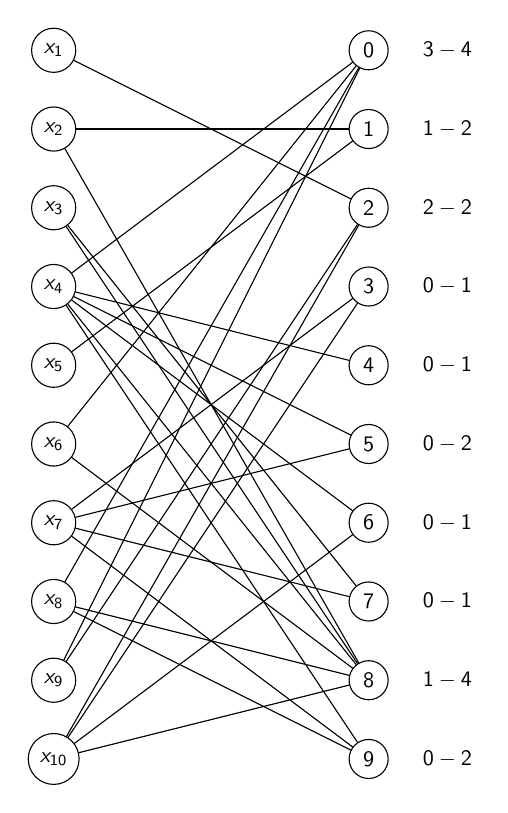
\begin{tikzpicture}[scale=1.0, every node/.style={scale=0.8}]
		\node[draw,circle] (x1)at(0,0) {$x_1$};
		\node[draw,circle] (x2)at(0,-1) {$x_2$};
		\node[draw,circle] (x3)at(0,-2) {$x_3$};
		\node[draw,circle] (x4)at(0,-3) {$x_4$};
		\node[draw,circle] (x5)at(0,-4) {$x_5$};
        \node[draw,circle] (x6)at(0,-5) {$x_6$};
        \node[draw,circle] (x7)at(0,-6) {$x_7$};
        \node[draw,circle] (x8)at(0,-7) {$x_8$};
        \node[draw,circle] (x9)at(0,-8) {$x_9$};
        \node[draw,circle] (x10)at(0,-9) {$x_{10}$};
        
		\node[draw,circle] (y0)at(4,0) {$0$};
		\node[draw,circle] (y1)at(4,-1) {$1$};
		\node[draw,circle] (y2)at(4,-2) {$2$};
        \node[draw,circle] (y3)at(4,-3) {$3$};
        \node[draw,circle] (y4)at(4,-4) {$4$};
        \node[draw,circle] (y5)at(4,-5) {$5$};
        \node[draw,circle] (y6)at(4,-6) {$6$};
        \node[draw,circle] (y7)at(4,-7) {$7$};
        \node[draw,circle] (y8)at(4,-8) {$8$};
        \node[draw,circle] (y9)at(4,-9) {$9$};
        
		\draw (x1) -- (y2);
        \draw (x2) -- (y1);
        \draw (x2) -- (y8);
        \draw (x3) -- (y7);
        \draw (x3) -- (y8);
        \draw (x4) -- (y0);
        \draw (x4) -- (y4);
        \draw (x4) -- (y5);
        \draw (x4) -- (y6);
        \draw (x4) -- (y8);
        \draw (x4) -- (y9);
        \draw (x5) -- (y1);
        \draw (x6) -- (y0);
        \draw (x6) -- (y8);
        \draw (x7) -- (y3);
        \draw (x7) -- (y5);
        \draw (x7) -- (y7);
        \draw (x7) -- (y9);
        \draw (x8) -- (y0);
        \draw (x8) -- (y8);
        \draw (x8) -- (y9);
        \draw (x9) -- (y0);
        \draw (x9) -- (y2);
        \draw (x10) -- (y2);
        \draw (x10) -- (y3);
        \draw (x10) -- (y6);
        \draw (x10) -- (y8);
        
        \node[draw=none] (b0)at (5,0) {$3-4$};
        \node[draw=none] (b1)at (5,-1) {$1-2$};
        \node[draw=none] (b2)at (5,-2) {$2-2$};
        \node[draw=none] (b3)at (5,-3) {$0-1$};
        \node[draw=none] (b4)at (5,-4) {$0-1$};
        \node[draw=none] (b5)at (5,-5) {$0-2$};
        \node[draw=none] (b6)at (5,-6) {$0-1$};
        \node[draw=none] (b7)at (5,-7) {$0-1$};
        \node[draw=none] (b8)at (5,-8) {$1-4$};
        \node[draw=none] (b9)at (5,-9) {$0-2$};
        
\end{tikzpicture}

\caption{A random instance of $gcc$ }
\label{randomInstance}
\end{figure}

\label{OrderInstantiationExample}
\end{example}

In order to measure how different is the behavior of these estimators within $maxSD$, we will use two measures of the similarity between two instantiation orders:
\noteGilles{Est-ce que ce sont des mesures maison? Si on considère pour chaque variable ses densités de solution comme une distribution discrète, il y a quelques mesures standard de similitude qu'on peut utiliser, dont la divergence de Kullback-Leibler. On prendrait ensuite la moyenne de cette divergence sur l'ensemble des variables.}
\begin{itemize}
\item[-] $m_{LP}(I_1, I_2)$ : the length of the common prefix between the instantiation order $I_1$ and $I_2$. The first instantiations are more important. We want to measure how many choices will be common in a row at the beginning. This measure is then normalized, dividing it by $n$.

\item[-] $m_{WS}(I_1, I_2)$ : the weighted sum of common elements between the instantiations order $I_1$ and $I_2$. It measures the number of common elements and favor the common elements that appear in the beginning . The weight of the $k^{th}$ elements among $p$ instantiations is $p-k+1$.

Let $I_1 = (\iota^1_1, \ldots, \iota^1_p)$, $I_2 = (\iota^2_1, \ldots, \iota^2_p)$ and $\chi$, the function such that $\chi(u,v)=1$ if $u=v$ and $\chi(u,v)=0$ otherwise. Then:

\begin{equation*}
	m_{WS}(I_1, I_2) = \frac{\sum_{k=1}^p (p-k+1)\cdot \chi(\iota^1_k, \iota^2_k)}{\frac{1}{2}\cdot p\cdot(p+1)}
\end{equation*}

The denominator is here to normalize the measure, so we can make the comparison between the two estimators on different instances of $gcc$.

\end{itemize}

% \begin{table}[H]
% \centering
% \begin{tabular}{|l|c|c|c|c|c|c|}
%     \hline
%     \multirow{2}{*}{Instantiation} & \multicolumn{3}{|c|}{Estimation of $\#$solutions} & \multicolumn{3}{|c|}{Solution density} \\
%     \cline{2-7}
%     & corrected bound & PQZ bound & exact & corrected bound & PQZ bound & exact\\
%     \hline
%    	$x_2 \rightarrow 1$ & 1262.24 & 52.59 & 59 & 34.4\% & 34.4\% & 41.8\% \\
%     $x_2 \rightarrow 8$ & 2411.40 & 100.47 & 82 & 65.6\% & 65.6\% & 58.2\%\\
%     \hline
%     $x_3 \rightarrow 7$ & 1173.76 & 48.91 & 47.0 & 32.7\% & 32.7\% & 33.3\% \\
%     $x_3 \rightarrow 8$ & 2411.40 & 100.47 & 94.0 & 67.3\% & 67.3\% & 66.7\% \\
%     \hline
%     $x_4 \rightarrow 0$ & 5088.24 & 424.02 & 83 & 97.6\% & 80.4\% & 58.9\% \\
%     $x_4 \rightarrow 4$ & 20.95 & 20.95 & 11 & 0.4\% & 4.0\% & 7.8\% \\
%     $x_4 \rightarrow 5$ & 20.95 & 20.95 & 11 & 0.4\% & 4.0\% & 7.8\% \\
%     $x_4 \rightarrow 6$ & 20.95 & 20.95 & 11 & 0.4\% & 4.0\% & 7.8\% \\
%     $x_4 \rightarrow 8$ & 39.75 & 19.87 & 14 & 0.8\% & 3.8\% & 9.9\% \\
%     $x_4 \rightarrow 9$ & 20.95 & 20.95 & 11 & 0.4\% & 4.0\% & 7.8\% \\
%     \hline
%     $x_6 \rightarrow 0$ & 11699.82 & 487.49 & 127 & 99.7\% & 96.1\% & 90.1\%\\
%     $x_6 \rightarrow 8$ & 39.75 & 19.87 & 14 & 0.3\% & 3.9\% & 9.9\%\\
%     \hline
%     $x_7 \rightarrow 3$ & 2542.91 & 211.91 & 37 & 34.7\% & 27.6\% & 26.2\%\\
%     $x_7 \rightarrow 5$ & 2542.91 & 211.91 & 40 & 34.7\% & 27.6\% & 28.4\%\\
%     $x_7 \rightarrow 7$ & 346.07 & 28.84 & 24 & 4.7\% & 3.8\% & 17.0\%\\
%     $x_7 \rightarrow 9$ & 1896.10 & 316.02 & 40 & 25.9\% & 41.1\% & 28.4\%\\
% 	\hline
%     $x_8 \rightarrow 0$ & 10181.07 & 424.21 & 116 & 99.4\% & 91.2\% & 82.3\%\\
%     $x_8 \rightarrow 8$ & 39.75 & 19.87 & 14 & 0.4\% & 4.3\% & 9.9\%\\
%     $x_8 \rightarrow 9$ & 20.95 & 20.95 & 11 & 0.2\% & 4.5\% & 7.8\%\\
% 	\hline
%    	$x_9 \rightarrow 0$ & 5286.00 & 220.25 & 108 & 96.9\% & 72.4\% & 76.6\% \\
%     $x_9 \rightarrow 2$ & 168.22 & 84.11 & 33 & 3.1\% & 27.6\% & 23.4\%\\
%     \hline
%     $x_{10} \rightarrow 2$ & 5286.00 & 220.25 & 108 & 98.6\% & 79.7\% & 76.6\% \\
%     $x_{10} \rightarrow 3$ & 15.15 & 15.15 & 8 & 0.3\% & 5.5\% & 5.7\% \\
%     $x_{10} \rightarrow 6$ & 20.95 & 20.95 & 11 & 0.4\% & 7.9\% & 7.8\% \\
%     $x_{10} \rightarrow 8$ & 39.75 & 19.87 & 14 & 0.7\% & 7.2\% & 9.9\% \\
%     \hline
    
    
%  \end{tabular}
% ~	\caption{Comparison of solution densities according to the bounds on the instance of $gcc$ presented in Figure \ref{randomInstance}}
%     \label{comparisonSolutionDensity}
% \end{table}

These two coefficients are normalized, such that if it is equal to 1, then the two instantiation orders are equal and, if it is equal to 0, they are very different. In Example \ref{exampleSimilarity}, we show how to compute these similarity coefficients.

\begin{example}
	Taking the three instantiations orders $I_{PQZ}$, $I_{Cor}$ ans $I_{exact}$ the instantiations orders given by the PQZ bound, the corrected bound and the exact computation in Example \ref{OrderInstantiationExample}.
    \noteGilles{On s'intéresse davantage aux mesures entre chacun et l'exact; est-ce qu'il est utile de mesurer entre les deux bornes?}
    \begin{itemize}
    \item[-] The length of the common prefix between the order given by the $PQZ$ bound and its correction is 2, then $m_{LP}(I_{PQZ}, I_{Cor}) = \frac{2}{25}= 8\%$. Also, we have $m_{LP}(I_{PQZ}, I_{exact}) = \frac{3}{25} = 12\%$, as only the first instantiation is identical and $m_{LP}(I_{PQZ}, I_{exact}) = 8\%$.
    
    \item[-] The instantiations $x_6 \rightarrow 0$, $x_8 \rightarrow 0$, $x_9 \rightarrow 0$, $x_3 \rightarrow 8$, $x_2 \rightarrow 8$, $x_4 \rightarrow 9$, $x_6 \rightarrow 8$  are in the same position in the ordering given by the PQZ bound and its correction. Their respective weight are : 26, 25, 22, 21, 20, 6 and 3. Then the weighted sum is 123 and we have $m_{WS}(I_{Cor}, I_{exact}) = \frac{123}{\sum_{k=1}^{25} k} = 37.8\%$. We also have $m_{WS}(I_{PQZ}, I_{exact}) = 25.2\%$ and $m_{WS}(I_{Cor}, I_{exact}) = 30.2\%$.
    
    \end{itemize}
	\label{exampleSimilarity}
\end{example}

Now that we have seen how to compare instantiations orders, we generate randomly 1000 instances of feasible $gcc$ and we will compare the orders given by the PQZ estimator, its correction and the exact computation. To generate those instances, we will apply the same method we used for the generation of the instance presented in Example \ref{OrderInstantiationExample} with the same parameters, $n=10, m=10$ and $p=0,3$.

Figure \ref{similarityLenghtCommonPrefix}a shows the number of instances in function of the percentage of similarity between the resulting instantiations orders given by the PQZ bound and its correction, according to the length of common prefix measure. We can notice that almost 600 among the 1000 generated instances, lead to less than 2\% similarity. More than 90\% of the instances are less than 20\% similar. The $PQZ$ bound and its correction very often lead to different instantiations orders. 
%
Figure \ref{similarityLenghtCommonPrefix}b shows the number of instances in function of the percentage of similarity between the resulting instantiations orders given by the exact computation and the two other estimators, according to the length of common prefix measure. The corrected bound is similar at less than 2\% to the exact bound for $58.9\%$ of all instances, and the PQZ bound for only $51.6\%$. %Both estimators are far from being similar to the order given by the exact computation. 
In general, the corrected bound gives more accurate instantiations orders.

\begin{figure}

	\begin{minipage}[c]{.46\linewidth}
     	 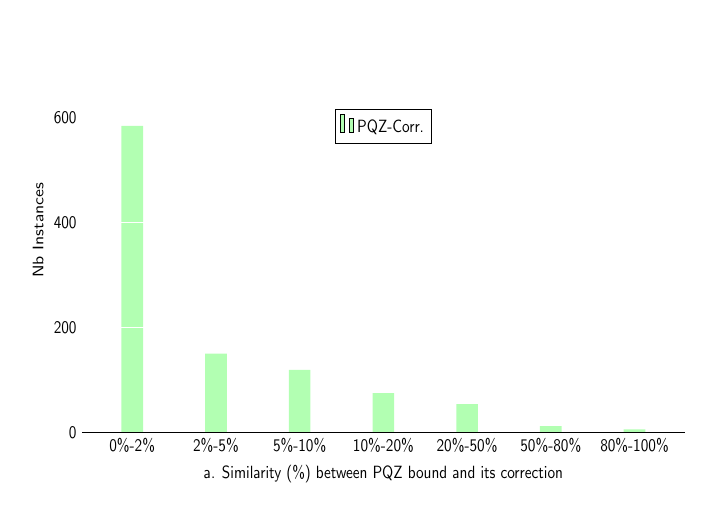
\begin{tikzpicture}[xscale=0.55, yscale=0.8, every node/.style={xscale=1, yscale=0.8}]
  \centering
  \begin{axis}[
        ybar, axis on top,
        height=8cm, width=15.5cm,
        bar width=0.5cm,
        ymajorgrids, tick align=inside,
        major grid style={draw=white},
        enlarge y limits={value=.1,upper},
        ymin=0, ymax=700,
        axis x line*=bottom,
        axis y line*=left,
        y axis line style={opacity=0},
        tickwidth=0pt,
        enlarge x limits=true,
        legend style={
            at={(0.5,0.8)},
            anchor=north,
            legend columns=-1,
            /tikz/every even column/.append style={column sep=0.5cm}
        },
        ylabel={Nb Instances},
        xlabel={a. Similarity (\%) between PQZ bound and its correction},
        symbolic x coords={0\%-2\%,2\%-5\%,5\%-10\%,10\%-20\%,20\%-50\%,50\%-80\%,80\%-100\%},
        xtick=data
    ]
    \addplot [draw=none,fill=green!30] coordinates {
      (0\%-2\%,584)(2\%-5\%,150)(5\%-10\%,119)(10\%-20\%,75)(20\%-50\%,54)(50\%-80\%,12)(80\%-100\%,6)
};

    \legend{PQZ-Corr.}
  \end{axis}
  \end{tikzpicture}
	\end{minipage} \hfill
	\begin{minipage}[c]{.46\linewidth}
     	 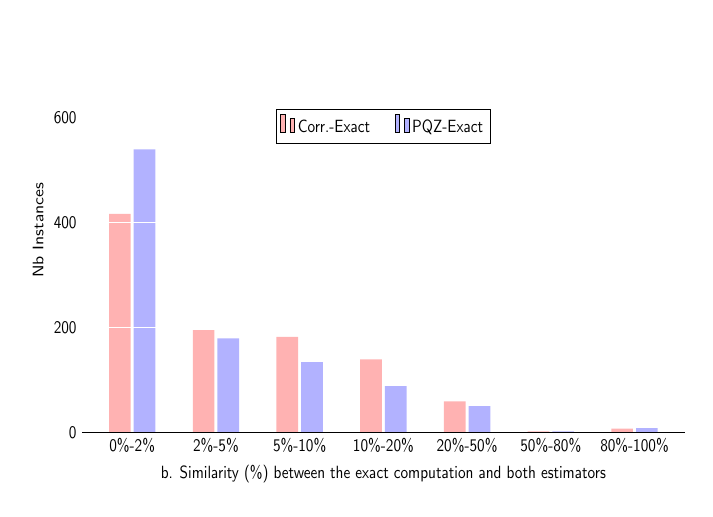
\begin{tikzpicture}[xscale=0.55, yscale=0.8, every node/.style={xscale=1, yscale=0.8}]
  \centering
  \begin{axis}[
        ybar, axis on top,
        height=8cm, width=15.5cm,
        bar width=0.5cm,
        ymajorgrids, tick align=inside,
        major grid style={draw=white},
        enlarge y limits={value=.1,upper},
        ymin=0, ymax=700,
        axis x line*=bottom,
        axis y line*=left,
        y axis line style={opacity=0},
        tickwidth=0pt,
        enlarge x limits=true,
        legend style={
            at={(0.5,0.8)},
            anchor=north,
            legend columns=-1,
            /tikz/every even column/.append style={column sep=0.5cm}
        },
        ylabel={Nb Instances},
        xlabel={b. Similarity (\%) between the exact computation and both estimators},
        symbolic x coords={0\%-2\%,2\%-5\%,5\%-10\%,10\%-20\%,20\%-50\%,50\%-80\%,80\%-100\%},
        xtick=data
    ]
    \addplot [draw=none,fill=red!30] coordinates {
      (0\%-2\%,416)(2\%-5\%,195)(5\%-10\%,182)(10\%-20\%,139)(20\%-50\%,59)(50\%-80\%,2)(80\%-100\%,7)
 };
    \addplot [draw=none, fill=blue!30] coordinates {
      (0\%-2\%,539)(2\%-5\%,179)(5\%-10\%,134)(10\%-20\%,88)(20\%-50\%,50)(50\%-80\%,2)(80\%-100\%,8)
};
   
      
    \legend{Corr.-Exact, PQZ-Exact}
  \end{axis}
  \end{tikzpicture}
  	 \end{minipage}
    \caption{Proportion of instances per percentage of similarity according to $m_{LP}$}
    \label{similarityLenghtCommonPrefix}
    
\end{figure}


In Figure \ref{similarityWCS}a, we represent the number of instances in function of the percentage of similarity according to the weighted sum of common elements measure. With the $m_{WS}$ measure, only about 100 instances have more than 50\% similarity between the PQZ bound and its correction. The instantiation orders remain quite different. 

In Figure \ref{similarityWCS}b is represented the similarity between the exact computation and the two estimators according to the weighted sum of common elements measure. Though the $m_{WS}$ is a much more flexible measure, there are still more than 100 instances that remain below 50\% of similarity for both estimators. The correction seems to give closer instantiation orders than the PQZ estimator, as there are about 100 instances more that are less than 2\% similar for the PQZ estimator and about 150 instances more that are between 20\% and 50\% similar for its correction.

Also, $maxSD$ is a strategy that choose the assignment with the highest density. We notice that, for 42.5\% of these 1000 instances, the PQZ estimator and its correction would choose the same first decision. For 59.3\% of the instances, the exact computation and the corrected estimator would choose the same first decision against 47.0\% for the exact computation and the PQZ estimator. And for 32.6\% of the instances, the three estimators would choose the same first decision.

\begin{figure}
  \begin{minipage}[c]{.46\linewidth}
     	 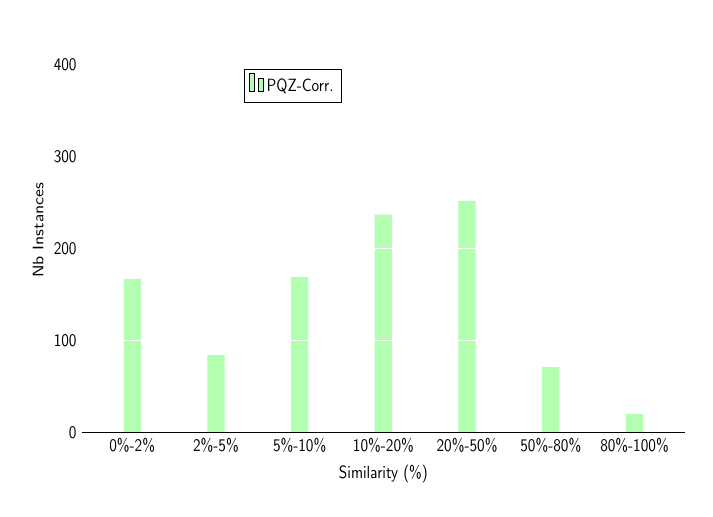
\begin{tikzpicture}[xscale=0.55, yscale=0.8, every node/.style={xscale=1, yscale=0.8}]
  \centering
  \begin{axis}[
        ybar, axis on top,
        height=8cm, width=15.5cm,
        bar width=0.4cm,
        ymajorgrids, tick align=inside,
        major grid style={draw=white},
        enlarge y limits={value=.1,upper},
        ymin=0, ymax=400,
        axis x line*=bottom,
        axis y line*=left,
        y axis line style={opacity=0},
        tickwidth=0pt,
        enlarge x limits=true,
        legend style={
            at={(0.35,0.9)},
            anchor=north,
            legend columns=-1,
            /tikz/every even column/.append style={column sep=0.5cm}
        },
        ylabel={Nb Instances},
        xlabel={Similarity (\%)},
        symbolic x coords={0\%-2\%,2\%-5\%,5\%-10\%,10\%-20\%,20\%-50\%,50\%-80\%,80\%-100\%},
        xtick=data
    ]
    \addplot [draw=none, fill=green!30] coordinates {
      (0\%-2\%,167)(2\%-5\%,84)(5\%-10\%,169)(10\%-20\%,237)(20\%-50\%,252)(50\%-80\%,71)(80\%-100\%,20)
};
    \legend{PQZ-Corr.}
  \end{axis}
  \end{tikzpicture}
	\end{minipage} \hfill
	\begin{minipage}[c]{.46\linewidth}
     	  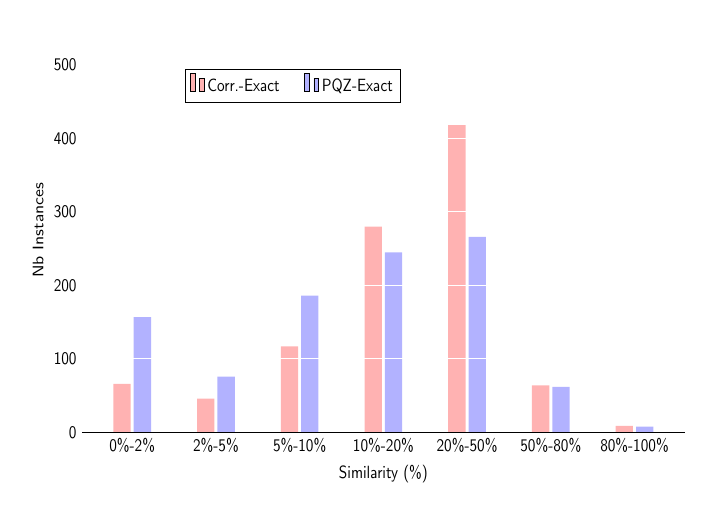
\begin{tikzpicture}[xscale=0.55, yscale=0.8, every node/.style={xscale=1, yscale=0.8}]
  \centering
  \begin{axis}[
        ybar, axis on top,
        height=8cm, width=15.5cm,
        bar width=0.4cm,
        ymajorgrids, tick align=inside,
        major grid style={draw=white},
        enlarge y limits={value=.1,upper},
        ymin=0, ymax=500,
        axis x line*=bottom,
        axis y line*=left,
        y axis line style={opacity=0},
        tickwidth=0pt,
        enlarge x limits=true,
        legend style={
            at={(0.35,0.9)},
            anchor=north,
            legend columns=-1,
            /tikz/every even column/.append style={column sep=0.5cm}
        },
        ylabel={Nb Instances},
        xlabel={Similarity (\%)},
        symbolic x coords={0\%-2\%,2\%-5\%,5\%-10\%,10\%-20\%,20\%-50\%,50\%-80\%,80\%-100\%},
        xtick=data
    ]
    \addplot [draw=none,fill=red!30] coordinates {
       (0\%-2\%,66)(2\%-5\%,46)(5\%-10\%,117)(10\%-20\%,280)(20\%-50\%,418)(50\%-80\%,64)(80\%-100\%,9)
};
    \addplot [draw=none, fill=blue!30] coordinates {
      (0\%-2\%,157)(2\%-5\%,76)(5\%-10\%,186)(10\%-20\%,245)(20\%-50\%,266)(50\%-80\%,62)(80\%-100\%,8)
};

    \legend{Corr.-Exact, PQZ-Exact}
  \end{axis}
  \end{tikzpicture}
  	\end{minipage}
    \caption{Proportion of instances per percentage of similarity according to $m_{WS}$}
    \label{similarityWCS}
\end{figure}



In this subsection, we have shown how to compare the influence of different number of solutions estimators within $maxSD$ on the instantiations ordering, and we have shown that the PQZ bound and its correction behave in a different way.

\noteGilles{Puisque maxSD ne s'intéresse vraiment qu'à l'affectation correspondant à la densité la plus élevée, il serait bon d'indiquer la proportion d'exemplaires où chaque estimateur choisirait la même affectation (et en tenant compte des densités max à égalité).}

\subsection{Performance analysis on generated instances}
\label{experimentalPerformance}

In this subsection we analyze the performance of each estimator within the $maxSD$ strategy. We generate random instances of varying degree of difficulty, on which we run the two variants of the $maxSD$ strategy. We first explain the generation process of such random instances and then we analyze the results obtained.

\subsubsection{Generation of random CSPs}

Let $n$ be the number of variables and $m$ the number of values. We consider that each variable can take any value, that is $\forall x_i \in X, D_i = \lbrace 0, \ldots, m-1 \rbrace$, thus the associated Value Graph is complete. Then, we add $n_C$ global cardinality constraints to this CSP. 
\noteGilles{puisque nous avons déjà $n$, $n_C$ ressemble à un produit; choisir une autre notation à une seule lettre}
The scope of each $gcc$ is chosen randomly : each variable has a $50\%$ chance to be picked. For each $gcc$, as the value graph is complete, we must generate occurrences constraint for every value $0, \ldots, m-1$. We are also given a tightness $\tau$, which defines the length of every occurrence interval of each value. Let $\lbrace x_{i_1}, \ldots, x_{i_q}\rbrace$ be the scope of one $gcc$, then the length of every occurrence interval of this $gcc$ is $\tau \cdot q$, rounded to the nearest integer. The generated $gcc$ are not trivially unsatisfiable, as we also ensure that the generated occurrence intervals, $[l_j, u_j]$, are such that:

\begin{equation*}
	\sum_{j=1}^m l_j \leq q \leq \sum_{j=1}^m u_j
\end{equation*}

We also ensure that any scope of a $gcc$ is not included in another $gcc$. Indeed, two such $gcc$ can be considered as one $gcc$, in which each occurrence interval is the intersection of two occurrence interval. We have thus exactly $n_C$ disjoint global cardinality constraints in the generated $CSP$. This is an important point as we want the number of $gcc$ and the tightness to be the two parameters that will directly affect the difficulty of the random instance.



\subsubsection{Results Analysis}

We generated several random CSP, with the method described above with the following parameters : $n=20, m=20$, $\tau \in [0.1,1]$ by step of $0.1$ and $n_C \in [2,10]$ by step of 1. For each couple $(\tau, n_C)$, we generate 50 random instances for a total of 4500 instances. We solve each instance with two different strategies: $maxSD$ with the PQZ bound and $maxSD$ with the corrected bound. The instances and the strategies are implemented in Choco solver \cite{chocoSolver} and we set, for each resolution, the time limit to 1 min and run on a 2.2GHz Intel Core i7 with 2.048GB.

The $maxSD$ heuristic proposes to compute an estimator of the solution density, for each possible remaining instantiation, each time a fixed point is reached. This is a very costly strategy. Here, we will only compute and store the solution densities in the beginning of the search and each time we reach a fixed point, we will refer to them and choose the instantiation that led to the highest solution density at the beginning of the search and that is still available.
\noteGilles{Puisque tous les domaines sont initialement complets, les densités calculées à la racine ne fournissent probablement pas d'information discriminante. D'autres heuristiques de branchement font sans doute tout aussi bien dans de telles circonstances?
Il faudrait au moins retirer des valeurs des domaines initiaux.}
\noteGilles{Pour l'efficacité, ce que nous avons proposé dans notre article à CPAIOR'18 est de recalculer seulement lorsque les domaines des variables dans la portée d'une contrainte ont suffisamment changé, mesuré simplement comme la somme de la taille des domaines.}
In Table \ref{nbSolved}, we give the number of instances that have been proved satisfiable or unsatisfiable by $maxSD$ with both estimators. For a given number of constraints, it seems that instances whose $gcc$ has a tightness between 0.3 and 0.8 are slightly harder than the other. This can be explained by the fact that, if the constraints are tighter, then it is easier to prove unsatisfiability, and if they are less tight, it is easier to find a solution. Though, for a given tightness, the number of constraints have a bigger influence on the instances difficulty and hardest instances seems to be instances with around 8 $gcc$. In the generated instances, the hardest instances are for the couple $(\tau = 0.6, n_C = 8)$.

In total, with the PQZ bound, we are able to solve 4370 instances over 4500, against 4248 instances for the corrected bound. The results are very comparable, even if the PQZ bound seems slightly better than its correction.

% In Table \ref{nbBacktracks} and Table \ref{resolutionTimes}, we present the number of backtracks and resolution times (in s) that have been required in average to solve each instance. It seems that the PQZ estimator performs slightly better than its correction in average. If we look at the couple $(\tau = 0.6, n_C = 8)$, the corrected bound needed less backtracks and less time to solve the corresponding instances, but globally, it does not seem like one estimator outperforms the other one. 

We now focus only on the instances that have been solved by both estimators. In Figure \ref{benchCloudPoints}a we compare the required number of backtracks for each instance that have been solved (proved satisfiable or unsatisfiable) with both estimators. Blue dots represent the satisfiable instances and red ones represent the unsatisfiable instances. We observe that there are a lot of red dots near the first bisector, which means that unsatisfiable instances roughly require the same number of backtracks with both estimators. For 80\% of the unsatisfiable instances, the ratio of the number of backtracks between the two estimators is inferior to 3.1 (inside the interval delimited by dots on Fig. \ref{benchCloudPoints}). %The blue dots are nearly equally distributed on both sides of the bisector. 
On the satisfiable instances, there are 660 blue points over bisector against 374 below. The PQZ estimator obtains better results on these satisfiable instances. 
%Some satisfiable instances are solved without performing any backtrack for one estimator, while it takes more backtracks for the other estimator. 
There are 179 satisfiable instances that are solved without backtracking for the PQZ estimator (represented by the blue dots on the ordinate axis, excepted the origin). And there are 88 satisfiable instances that require no backtrack for the corrected estimator. There are also 965 blue points and 451 red points at the origin, in which case the corresponding instances were solved by propagation, without backtracking.

%XXX Quantifier les points rouges dans les zones : noire, au dessus hors zone noire, au dessous hors zone noire, axes et origine.
%XXX Distinction sat / unsat : l'heuristique est faite plutôt pour les sat. Sur les problèmes unsat, c'est quasi pareil pour les deux heuristiques.
%XXX Sur les problèmes sat : c'est ce pour quoi est fait l'heuristique. PQZ est un estimateur, pas une borne, donc dans le cas où il y a beaucoup de solutions il "force" plus que la borne. Utilisé comme estimateur, il conserve un grand intérêt heuristique.


On Figure \ref{benchCloudPoints}b, we compare the resolution time for each instance that has been solved with both estimators in a similar way. For some instances, it is very quick to prove satisfiability or unsatisfiability: almost 15\% of the instances require less than 0.1s to be solved. Again, we  observe that the unsatisfiable instances are closer to the bisector : 80\% of the unsatisfiable instances are such that the ratio between the solving time with PQZ and the solving time with its correction is inferior to 2.3 . As for the satisfiable instances, they are again more widely distributed. There are 839 blue points below the bisector and 1160 above. %To conclude on this benchmark, the two estimators have very similar performance. The PQZ estimator is a little better on satisfiable instances, but globally, it does not seem like one estimator outperforms the other one.

Our conclusions on this benchmark are the following. As a preliminary remark, both heuristics are meant to tune the search toward areas with many solutions (or a high solution density for the $gcc$ constraints). The heuristics are not meant to provoke failures, hence, there are not suited to unsatisfiable instances. In practice, we observe on the benchmark that both heuristics roughly behave the same on unsatisfiable instances, with both a number of backtracks and a resolution time with a similar ratio (inside the black lines) on 80\% of the instances (red dots). On the satisfiable instances (blue dots), we observe that the PQZ heuristic is better than the Corrected heuristic. As proved in the previous sections, the PQZ is not based on a bound, but our experiments show that in practice it can be considered as an estimator of the solution density. In practice, on our benchmark, this estimator seems to be useful to guide the search. 
%
We observe that the heuristic based on the PQZ estimator pushes the search to choose different assignments of our correction based on an upper bound (cf Figures~\ref{similarityLenghtCommonPrefix} and~\ref{similarityWCS}). We assume that the quality of the PQZ results on the SAT instances is probably related to the fact that the artificial amplification of the PQZ estimator, to choose some assignment, still pushes the search into areas that most likely contain at least one solution.
%
However, in the end, no heuristic clearly dominates the other, the number of solved instances being quite distributed around the bisector.
  

In conclusion, on all these experiments, there is no clear dominance of the PQZ estimator over our upper bound, when they are used inside a $maxSD$ heuristic, in terms of solving efficiency. Nevertheless, we observe that there is a clear difference between them, when they are used to find an instantiation order. In addition, we also observed that the bug in the PQZ bound indeed happens, in which case the presumed upper bound gives a value below the exact number of solutions. In the end, the benchmark is conclusive on this precise matter: the PQZ estimator and our Corrected bound are not equivalent, although using them in $maxSD$ does not reveal this on the solving time.


%%%%%%%%%%%%%%%%%%%%%%%%%%%%%%%%%%%

\section{Conclusion}
This paper revisited the solution-counting strategies for the well-known global cardinality constraint. It first highlights that in the computation of the initial result provided by~\cite{PesantQZ12}, a solution can be counted several times and, thus, is not an upper bound. We also provide a correct calculation of such an upper bound. Finally, we build a benchmark for the $gcc$ constraint with a original method, which had not been done in the previous work, and we compare heuristics based on both quantities (the previous calculation by \cite{PesantQZ12} and our upper bound) on this benchmark. We first show that the two estimators lead to different choices within counting-based strategies. Finally, we solve a number of instances with both heuristics and compare the results. In practice, the heuristics based on \cite{PesantQZ12} calculation performs slightly better on our benchmark: although it is not a upper bound, it is proved useful as an \textit{estimator} of the solution density.

 Though the former result is not an upper bound, it remains an estimator that can be used to guide the search. That is probably why the error was difficult to spot. It also reinforces the idea that the correlation between one estimator and the actual number of solutions is much more important that its accuracy. A future work on $\texttt{global\_cardinality}$ could be to determines other estimators based, for example, on probabilistic approaches.
 
 %The main issue of those estimators on $\texttt{global\_cardinality}$ constraints, is that they require a lot of complex operations. Every instantiation for each constraint is tested and propagated. Computing them each time a decision has to be made is very time consuming. Indeed, we need to compute the Lower Bound Graph, the Upper Bound Graph then we need to estimate the number of matchings on these graphs. This is why, in the presented experiments, the instantiations ordering is only made in the beginning of the search. Thus, at each branch of the search tree, we do not necessarily visit first the space where there are more solutions at this point of the search. That is why estimators that are faster to compute are needed for this constraint. 
 
 
 

 
 







% \begin{table}[H]
%   		\begin{tabular}{|c|c|c|c|c|c|c|}
% \hline
% $\tau \backslash n_C$ & 2 & 3 & 4 & 5 & 6 \\
% \hline
% $\tau$ = 0.1 & 16874/\textbf{16795} & \textbf{17093}/24798 & 46940/\textbf{41905} & \textbf{17765}/19948 & \textbf{65518}/78460 \\
% \hline
% $\tau$ = 0.2 & \textbf{1011}/1214 & \textbf{19971}/33476 & \textbf{9188}/17973 & 19493/\textbf{18515} & \textbf{73860}/75259 \\
% \hline
% $\tau$ = 0.3 & 736/\textbf{278} & 131877/\textbf{22725} & \textbf{53607}/88541 & \textbf{64864}/149811 & 122751/\textbf{59915} \\
% \hline
% $\tau$ = 0.4 & \textbf{17}/30 & \textbf{17772}/39408 & \textbf{38808}/111706 & \textbf{67338}/102362 & \textbf{49471}/107863 \\
% \hline
% $\tau$ = 0.5 & \textbf{648}/803 & 130661/\textbf{46689} & 40951/\textbf{22404} & 122356/\textbf{57701} & 223113/\textbf{97272} \\
% \hline
% $\tau$ = 0.6 & \textbf{4805}/10545 & \textbf{8635}/9190 & 37886/\textbf{31321} & \textbf{81963}/176339 & \textbf{57430}/143473 \\
% \hline
% $\tau$ = 0.7 & 5446/\textbf{2022} & \textbf{13569}/81122 & \textbf{29257}/121320 & \textbf{106917}/163715 & \textbf{64351}/124762 \\
% \hline
% $\tau$ = 0.8 & 13463/\textbf{704} & \textbf{67724}/100239 & \textbf{74152}/145502 & \textbf{24953}/63467 & \textbf{72835}/94480 \\
% \hline
% $\tau$ = 0.9 & \textbf{3053}/3354 & \textbf{19703}/44054 & 111617/\textbf{91500} & \textbf{68538}/125215 & \textbf{95945}/231803 \\
% \hline
% $\tau$ = 1.0 & \textbf{822}/5964 & \textbf{6264}/67525 & \textbf{50745}/155688 & \textbf{89871}/100491 & \textbf{17453}/45512 \\
% \hline
% \end{tabular}
        
%         \vspace{10pt}

%     \begin{tabular}{|c|c|c|c|c|}
% \hline
% $\tau \backslash n_C$ & 7 & 8 & 9 & 10 \\
% \hline
% $\tau$ = 0.1 & 45809/\textbf{45564} & 25388/\textbf{23987} & \textbf{7234}/8807 & 2522/\textbf{2036} \\
% \hline
% $\tau$ = 0.2 & 146989/\textbf{127718} & \textbf{72564}/75276 & \textbf{82423}/121545 & 38540/\textbf{32194} \\
% \hline
% $\tau$ = 0.3 & 86875/\textbf{69420} & \textbf{45595}/49085 & \textbf{91121}/93349 & 34542/\textbf{29982} \\
% \hline
% $\tau$ = 0.4 & 136707/\textbf{98040} & 83497/\textbf{65517} & \textbf{21648}/24188 & \textbf{30850}/54515 \\
% \hline
% $\tau$ = 0.5 & \textbf{32642}/69050 & \textbf{96252}/110973 & 132173/\textbf{58807} & 60144/\textbf{59599} \\
% \hline
% $\tau$ = 0.6 & \textbf{41175}/52601 & 39161/\textbf{31454} & 73988/\textbf{63674} & \textbf{3171}/10922 \\
% \hline
% $\tau$ = 0.7 & 95958/\textbf{39342} & \textbf{83913}/127683 & \textbf{73196}/104150 & \textbf{71368}/93454 \\
% \hline
% $\tau$ = 0.8 & \textbf{98469}/143748 & \textbf{45162}/85131 & \textbf{61938}/95387 & 85792/\textbf{32468} \\
% \hline
% $\tau$ = 0.9 & \textbf{87347}/87640 & \textbf{62045}/78019 & 57122/\textbf{33778} & \textbf{56826}/89137 \\
% \hline
% $\tau$ = 1.0 & \textbf{30318}/167714 & \textbf{97745}/122929 & \textbf{104808}/112442 & \textbf{13880}/24393 \\
% \hline
% \end{tabular}
%         \caption{Number of backtracks in average on solved instances for both estimators (PQZ/Corr.) for each couple $(\tau, n_C)$}
%     \label{nbBacktracks}
% 	\end{table}




% \begin{table}[H]        
%     \begin{tabular}{|c|c|c|c|c|c|c|c|}
% \hline
% $\tau \backslash n_C$ & 2 & 3 & 4 & 5 & 6 & 7\\
% \hline
% $\tau$ = 0.1 & 0.11/\textbf{0.1} & \textbf{0.29}/0.43 & 0.97/\textbf{0.9} & \textbf{0.64}/0.69 & \textbf{1.7}/2.27 & 1.4/\textbf{1.35} \\
% \hline
% $\tau$ = 0.2 & \textbf{0.02}/0.03 & \textbf{0.38}/0.61 & \textbf{0.28}/0.48 & 0.59/\textbf{0.45} & 2.56/\textbf{2.51} & 5.15/\textbf{4.62} \\
% \hline
% $\tau$ = 0.3 & 0.01/0.01 & 1.42/\textbf{0.25} & \textbf{1.08}/1.73 & \textbf{1.46}/3.89 & 3.8/\textbf{2.17} & 3.1/\textbf{2.52} \\
% \hline
% $\tau$ = 0.4 & 0.01/0.01 & \textbf{0.43}/0.91 & \textbf{0.57}/2.38 & \textbf{1.88}/2.58 & \textbf{1.61}/3.71 & 4.68/\textbf{3.21} \\
% \hline
% $\tau$ = 0.5 & 0.01/0.01 & 1.59/\textbf{0.93} & 0.92/\textbf{0.39} & 2.48/\textbf{1.29} & 6.26/\textbf{3.25} & \textbf{1.07}/2.78 \\
% \hline
% $\tau$ = 0.6 & \textbf{0.07}/0.08 & \textbf{0.09}/0.12 & 1.1/\textbf{0.47} & \textbf{1.59}/3.85 & \textbf{1.84}/2.52 & 1.87/\textbf{1.84} \\
% \hline
% $\tau$ = 0.7 & 0.09/\textbf{0.03} & \textbf{0.29}/1.59 & \textbf{0.79}/2.39 & \textbf{3.5}/4.56 & \textbf{2.73}/3.69 & 3.88/\textbf{1.38} \\
% \hline
% $\tau$ = 0.8 & 0.18/\textbf{0.02} & \textbf{0.93}/1.23 & 1.5/\textbf{1.43} & \textbf{0.62}/1.22 & \textbf{1.84}/2.59 & \textbf{3.51}/4.82 \\
% \hline
% $\tau$ = 0.9 & \textbf{0.06}/0.07 & \textbf{0.32}/0.66 & 1.97/\textbf{1.93} & \textbf{2.05}/3.07 & \textbf{2.72}/6.09 & \textbf{3.3}/3.48 \\
% \hline
% $\tau$ = 1.0 & \textbf{0.02}/0.05 & \textbf{0.08}/0.6 & \textbf{1.34}/3.97 & 2.53/\textbf{2.24} & \textbf{0.71}/1.24 & \textbf{1.08}/5.36 \\
% \hline

%     \end{tabular}
    
%     \vspace{10pt}

% \begin{tabular}{|c|c|c|c|}
% \hline
% $\tau \backslash n_C$ & 8 & 9 & 10 \\
% \hline
% $\tau$ = 0.1 & 1.03/\textbf{1.01} & \textbf{0.34}/0.4 & 0.16/\textbf{0.14} \\
% \hline
% $\tau$ = 0.2 & 3.28/\textbf{3.19} & \textbf{3.98}/5.94 & 2.23/\textbf{1.93} \\
% \hline
% $\tau$ = 0.3 & \textbf{2.31}/2.65 & \textbf{2.65}/4.27 & 2.17/\textbf{2.12} \\
% \hline
% $\tau$ = 0.4 & 3.14/\textbf{2.63} & \textbf{1.06}/1.07 & \textbf{1.86}/3.29 \\
% \hline
% $\tau$ = 0.5 & 5.04/\textbf{4.71} & 6.71/\textbf{2.77} & \textbf{3.21}/3.5 \\
% \hline
% $\tau$ = 0.6 & 1.98/\textbf{1.15} & \textbf{3.42}/4.04 & \textbf{0.2}/0.68 \\
% \hline
% $\tau$ = 0.7 & \textbf{3.79}/5.44 & \textbf{3.39}/4.96 & \textbf{4.29}/5.71 \\
% \hline
% $\tau$ = 0.8 & \textbf{1.99}/4.02 & \textbf{3.36}/4.43 & 4.73/\textbf{1.92} \\
% \hline
% $\tau$ = 0.9 & \textbf{2.65}/3.25 & 3.09/\textbf{1.96} & \textbf{3.2}/5.35 \\
% \hline
% $\tau$ = 1.0 & \textbf{5.08}/5.51 & \textbf{4.91}/5.57 & \textbf{0.91}/1.73 \\
% \hline

% \end{tabular}
     
%         \caption{Resolution time (in s) in average on solved instances for both estimators (PQZ/Corr.) for each couple $(\tau, n_C)$}
%     \label{resolutionTimes}
    
% 	\end{table}
 
 

 
\bibliography{jairbugfix}
\bibliographystyle{theapa}

\end{document}








